%----------------------------------------------------------------------------------------
%	PACKAGES AND OTHER DOCUMENT CONFIGURATIONS
%----------------------------------------------------------------------------------------

\documentclass[
10pt, % Main document font size
a4paper, % Paper type, use 'letterpaper' for US Letter paper
oneside, % One page layout (no page indentation)
%twoside, % Two page layout (page indentation for binding and different headers)
pdfspacing, % Makes use of pdftex’ letter spacing capabilities via the microtype package
headinclude,
%footinclude, % Extra spacing for the header and footer
BCOR5mm, % Binding correction
ngerman, %set document to German
bibtotocnumbered,
]{scrartcl}
%{scrartcl}

%%%%%%%%%%%%%%%%%%%%%%%%%%%%%%%%%%%%%%%%%
% Arsclassica Article
% Structure Specification File
%
% This file has been downloaded from:
% http://www.LaTeXTemplates.com
%
% Original author:
% Lorenzo Pantieri (http://www.lorenzopantieri.net) with extensive modifications by:
% Vel (vel@latextemplates.com)
%
% License:
% CC BY-NC-SA 3.0 (http://creativecommons.org/licenses/by-nc-sa/3.0/)
%
%%%%%%%%%%%%%%%%%%%%%%%%%%%%%%%%%%%%%%%%%

%----------------------------------------------------------------------------------------
%	REQUIRED PACKAGES
%----------------------------------------------------------------------------------------

\usepackage[usenames,dvipsnames]{color} % Required for specifying custom colors and referring to colors by name

\usepackage[
nochapters, % Turn off chapters since this is an article        
beramono, % Use the Bera Mono font for monospaced text (\texttt)
%eulermath,% Use the Euler font for mathematics
eulerchapternumbers,
pdfspacing, % Makes use of pdftex’ letter spacing capabilities via the microtype package
dottedtoc % Dotted lines leading to the page numbers in the table of contents
]{classicthesis} % The layout is based on the Classic Thesis style

%\usepackage{arsclassica} % Modifies the Classic Thesis package

\usepackage[T1]{fontenc} % Use 8-bit encoding that has 256 glyphs

\usepackage[utf8]{inputenc} % Required for including letters with accents

\usepackage{graphicx} % Required for including images
\graphicspath{{Figures/}} % Set the default folder for images

\usepackage{enumitem} % Required for manipulating the whitespace between and within lists

\usepackage{lipsum} % Used for inserting dummy 'Lorem ipsum' text into the template

\usepackage{amsmath,amssymb,amsthm} % For including math equations, theorems, symbols, etc

\usepackage{varioref} % More descriptive referencing

\usepackage{url}

\usepackage{hyperref}

\usepackage{gensymb}	%for the \degree command

\usepackage[ngerman, english]{babel}

\usepackage[square,
authoryear,
%numbers,
longnamesfirst
]{natbib}

\usepackage{enumitem}

\usepackage{authblk}

\usepackage{relsize, etoolbox, lmodern}% http://ctan.org/pkg/{relsize,etoolbox}

\AtBeginEnvironment{quote}{\smaller\fontfamily{lmss}\selectfont}% Step font down one size relative to current font.
% see http://tex.stackexchange.com/questions/25249/how-do-i-use-a-particular-font-for-a-small-section-of-text-in-my-document for fontfamilies

\usepackage{chngcntr}

% to have a separation in the text with extra space between paragraphs and no indendation following
\newcommand*{\skippingparagraph}{\par\vspace{1.0\baselineskip}\noindent}

%----------------------------------------------------------------------------------------
%	HYPERLINKS
%---------------------------------------------------------------------------------------
\definecolor{mediumviolet-red}{rgb}{0.78, 0.08, 0.52}
\hypersetup{
%	draft, % Uncomment to remove all links (useful for printing in black and white)
	colorlinks=true, breaklinks=true, bookmarks=true,bookmarksnumbered,
	urlcolor=webbrown, linkcolor=mediumviolet-red, citecolor=webgreen, % Link colors
	pdftitle={}, % PDF title
	pdfauthor={\textcopyright}, % PDF Author
	pdfsubject={}, % PDF Subject
	pdfkeywords={}, % PDF Keywords
	pdfcreator={pdfLaTeX}, % PDF Creator
	pdfproducer={LaTeX with hyperref and ClassicThesis} % PDF producer
}

%----------------------------------------------------------------------------------------
%	TODONOTES
%---------------------------------------------------------------------------------------

\usepackage[colorinlistoftodos]{todonotes}

\newcommand{\todoInfo}[1]{\todo[color=blue!25]{INFO: #1}}
\newcommand{\todoCite}[1]{\todo[color=green!40]{INFO: #1}}


%----------------------------------------------------------------------------------------
%	CODESNIPPETS
%---------------------------------------------------------------------------------------

%%%%%%%%%%%%%%%%%%%%%%%%%%%%%%%%%%%%%%%%%
% Code Snippet
% LaTeX Template
% Version 1.0 (14/2/13)
%
% This template has been downloaded from:
% http://www.LaTeXTemplates.com
%
% Original author:
% Velimir Gayevskiy (vel@latextemplates.com)
%
% License:
% CC BY-NC-SA 3.0 (http://creativecommons.org/licenses/by-nc-sa/3.0/)
%
%%%%%%%%%%%%%%%%%%%%%%%%%%%%%%%%%%%%%%%%%
\usepackage{listings} % Required for inserting code snippets

\definecolor{DarkGreen}{rgb}{0.0,0.4,0.0} % Comment color
\definecolor{highlight}{RGB}{255,251,204} % Code highlight color
\definecolor{DogwoodRose}{rgb}{0.84, 0.09, 0.41}
\definecolor{lemonchiffon}{rgb}{1.0, 0.98, 0.8}
\definecolor{lightgoldenrodyellow}{rgb}{0.98, 0.98, 0.82}
\definecolor{oldlace}{rgb}{0.99, 0.96, 0.9}
\definecolor{oldlavender}{rgb}{0.47, 0.41, 0.47}
\definecolor{pakistangreen}{rgb}{0.0, 0.4, 0.0}
\definecolor{ao}{rgb}{0.0, 0.0, 1.0}
\definecolor{britishracinggreen}{rgb}{0.0, 0.26, 0.15}
\definecolor{coquelicot}{rgb}{1.0, 0.22, 0.0}
\definecolor{cordovan}{rgb}{0.54, 0.25, 0.27}
\definecolor{darkcandyapplered}{rgb}{0.64, 0.0, 0.0}
\definecolor{mediumchampagne}{rgb}{0.95, 0.9, 0.67}

\lstdefinestyle{Style1}{ % Define a style for your code snippet, multiple definitions can be made if, for example, you wish to insert multiple code snippets using different programming languages into one document
	language=JavaScript, % Detects keywords, comments, strings, functions, etc for the language specified
	backgroundcolor=\color{oldlace}, % Set the background color for the snippet - useful for highlighting
	basicstyle=\smaller\smaller\ttfamily, % The default font size and style of the code
	breakatwhitespace=true, % If true, only allows line breaks at white space
	breaklines=true, % Automatic line breaking (prevents code from protruding outside the box)
	captionpos=b, % Sets the caption position: b for bottom; t for top
	commentstyle=\usefont{T1}{pcr}{m}{sl}\color{ao}, % {m}DarkGreen Style of comments within the code - dark green courier font
	deletekeywords={}, % If you want to delete any keywords from the current language separate them by commas
	%escapeinside={\%}, % This allows you to escape to LaTeX using the character in the bracket
	firstnumber=1, % Line numbers begin at line 1
	frame=single, % Frame around the code box, value can be: none, leftline, topline, bottomline, lines, single, shadowbox
	frameround=tttt, % Rounds the corners of the frame for the top left, top right, bottom left and bottom right positions
	keywordstyle=\color{darkcandyapplered}\textbf, % Functions are bold and blue
	morekeywords={}, % Add any functions no included by default here separated by commas
	numbers=left, % Location of line numbers, can take the values of: none, left, right
	numbersep=10pt, % Distance of line numbers from the code box
	numberstyle=\tiny\color{Gray}, % Style used for line numbers
	rulecolor=\color{black}, % Frame border color
	showstringspaces=false, % Don't put marks in string spaces
	showtabs=false, % Display tabs in the code as lines
	stepnumber=5, % The step distance between line numbers, i.e. how often will lines be numbered
	stringstyle=\color{Purple}, % Strings are purple
	tabsize=2, % Number of spaces per tab in the code
}

\definecolor{darkgray}{rgb}{.4,.4,.4}
\definecolor{purple}{rgb}{0.65, 0.12, 0.82}


%define Javascript language
\lstdefinelanguage{JavaScript}{
	keywords={typeof, new, true, false, catch, try, finally, function, return, null, then, catch, switch, var, if, in, while, do, else, case, break, yield, async, await},
	keywordstyle=\color{blue}\bfseries,
	ndkeywords={class, export, boolean, throw, implements, import, this},
	ndkeywordstyle=\color{darkgray}\bfseries,
	identifierstyle=\color{black},
	sensitive=false,
	comment=[l]{//},
	morecomment=[s]{/*}{*/},
	commentstyle=\color{purple}\ttfamily,
	stringstyle=\color{red}\ttfamily,
	morestring=[b]',
	morestring=[b]"
}

\lstset{
	language=JavaScript,
	extendedchars=true,
	basicstyle=\footnotesize\ttfamily,
	showstringspaces=false,
	showspaces=false,
	numbers=left,
	numberstyle=\footnotesize,
	numbersep=9pt,
	tabsize=2,
	breaklines=true,
	showtabs=false,
	captionpos=b
}

% Create a command to cleanly insert a snippet with the style above anywhere in the document
\newcommand{\insertcode}[2]{\begin{itemize}\item[]\lstinputlisting[{caption={#2}},label=#1,style=Style1]{#1}\end{itemize}} % The first argument is the script location/filename and the second is a caption for the listing
 % Include the structure.tex file which specified the document structure and layout

%\documentclass[10pt,a4paper]{report}

%----------------------------------------------------------------------------------------
%	TITLE AND AUTHOR(S)
%----------------------------------------------------------------------------------------
\selectlanguage{ngerman}

\subtitle{\normalfont{Fachpraktikum 1597 an der FernUni Hagen im SS 2017:\protect\\Parallele Programmierung }}

\title{\normalfont{Abschlussbericht zur Erkennung von möglichen Notlandefeldern aus Höhendaten mittels POSIX Thread Implementation}} % The article title

\author{Felix Eckstein*, Dr. Björn Wittich**} % The article author(s) 

\date{August 2017} % An optional date to appear under the author(s)

%----------------------------------------------------------------------------------------


                


\begin{document}

	\maketitle % Print the title/author/date block

	\tableofcontents % Print the table of contents

	
	{\let\thefootnote\relax\footnotetext{* \textit{Student im Bachelor of Science Informatik an der FernUniversität Hagen,\protect\\Matr.-\#: 8161569, \href{mailto:felix.eckstein@gmx.de}{felix.eckstein@gmx.de}}}}
	{\let\thefootnote\relax\footnotetext{** \textit{Student im Bachelor of Science Informatik an der FernUniversität Hagen,\protect\\Matr.-\#: 9265953, \href{mailto:BjoernWittich@gmx.de}{BjoernWittich@gmx.de}}}}
	
	\selectlanguage{ngerman}

\section{Aufgabenstellung}

Im Rahmen des Praktikums sind aus Geoterraindaten mögliche Notlandebahnen für Notfallsituationen im Luftverkehr zu ermitteln. Im Falle eines vollständigen Turbinenausfalls kann es z.B. vorkommen, dass der nächstgelegene Flughafen auf Grund aktueller Flughöhe und Windrichtung nicht mehr erreicht werden kann.

Innerhalb der zur Verfügung gestellten Geländedaten, die im GeoTiff Format vorliegen, soll ein Algorithmus entwickelt werden, der plane Flächen darin ermittelt, die sich zum Landen eines Flugzeugs eignen.

Die Eignung einer Landebahn ergibt sich aus Parametern wie Länge, Breite, Winkel, Steigung, Holprigkeit und Querneigung der Bahn.
Diese werden der Software zur Ermittlung mitgegeben, welche den Kriterien entsprechende Landebahnen findet.
Insbesondere Breite und Länge der Landebahn müssen konfigurierbar sein, da ein Ultraleichtflugzeug und eine Verkehrsmaschine wie ein Airbus A380 oder eine Boeing 767 völlig unterschiedliche Vorgaben benötigen.

Weiterhin ist der Winkel der Bahn im Zusammenspiel mit den aktuell vorherrschenden Windverhältnissen von großer Bedeutung. 
Ein weiterer Fokus dieses Praktikums liegt in der Anwendung von Parallelverarbeitung.

Im Speziellen soll eine Parallelisierung der Landebahnsuche mit \texttt{p\_threads}, einer klassische Shared Memory Architektur, durchgeführt werden.
Es soll untersucht werden, wie sich der Speed-up mit zunehmender Anzahl an Threads verhält und mit der seriellen Abarbeitung verglichen werden.

Die gefundenen Landebahnen sind anschließend in einem User Interface (UI) zu visualisieren.

Die Software soll dem Piloten eine Entscheidungshilfe sein und mögliche Optionen anbieten. Insbesondere die Kombination von Notfall und der teilweise stark eingeschränkten Sicht im Cockpit soll in solch einem Fall eine technische Unterstützung die Entscheidungsfindung erleichtert werden.
Die Landung selbst soll nach wie vor von einem Menschen durchgeführt werden. Fragestellungen wie Fahrwerk ein- oder ausfahren bleiben hier außen vor.     

\section{Architektur}

Zur Lösung der Aufgabenstellung muss zunächst eine Systemarchitektur festgelegt werden.

\subsection{Überblick}
Zum Einlesen der Rohdaten, Steuern der Applikation und zum Auffinden, Persistieren und Anzeigen der potentiellen Notlandefelder sind vielfältige Schritte notwendig. Diese haben jeweils ihre eigenen spezifischen Herausforderungen und sind bei näherer Betrachtung sogar relativ unabhängig voneinander lösbar.

Daraus ergibt sich die Möglichkeit, dass System aus relativ lose gekoppelten Komponenten aufzubauen, welche jeweils in einer Programmiersprache ent\-wickelt werden, die auf die jeweilige Aufgabe abgestimmt, ihre Stärken ausspielen kann. In der vorliegenden Aufgabenstellung wurde entschieden, die Aufgaben, welche vornehmlich große Datenmengen bewegen und "`Number Crunching"' betreiben in C/C++ zu implementieren, während Datenbankzugriffe und das UI in JavaScript realisiert wurden.

Eine grobe Übersicht über die einzelnen Systemkomponenten bietet Abbildung \ref{architektur}.

\begin{figure}[h]
	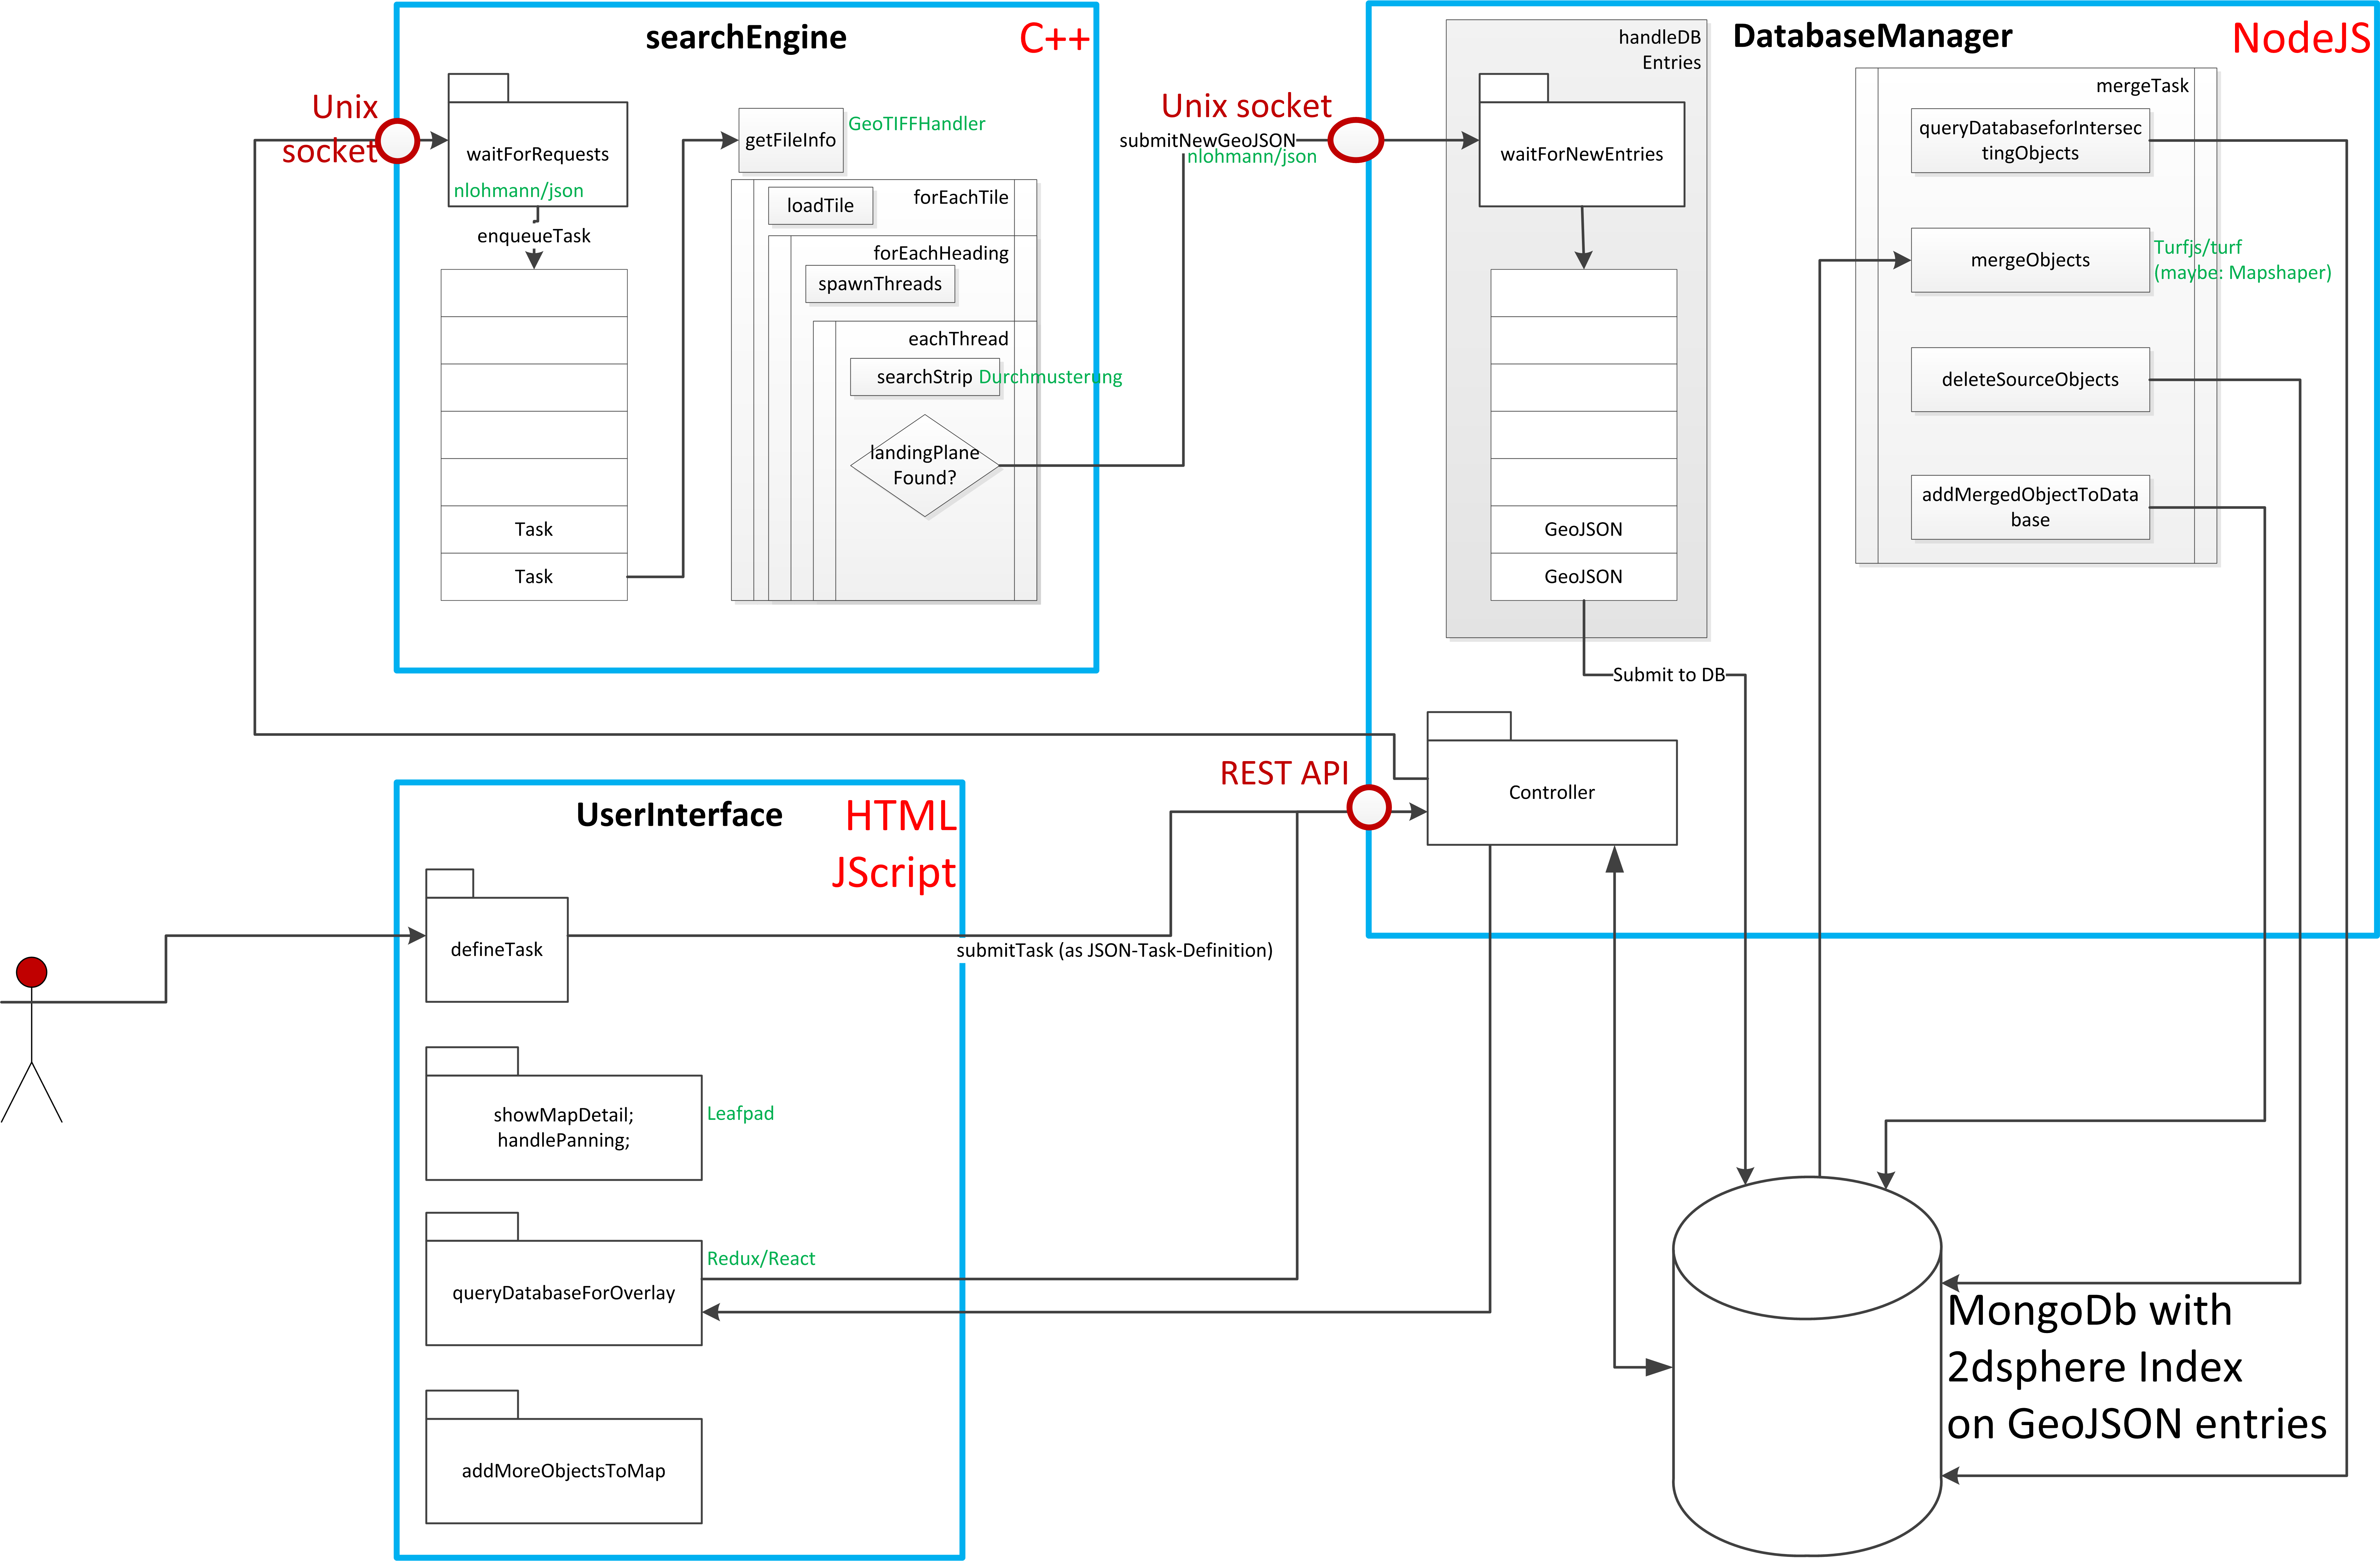
\includegraphics[width=\textwidth]{../Architektur/Architektur.png}
	\caption{Architekturüberblick} \label{architektur}
\end{figure}

Hier sind vier unabhängige Komponenten zu erkennen:
\begin{itemize}
	\item das UserInterface (UI)
	\item der DatabaseManager (DBM)
	\item die SearchEngine (SE)
	\item die Datenbank (DB)
\end{itemize}

Abgebildet auf eine Model-View-Controller-Architektur (MVC) würde das User Interface der View entsprechen, der Database Manager dem Controller, die Datenbank dem Model. Die Search Engine ist der Geschäftslogik zuzuordnen und kommuniziert ausschließlich über den Controller.
In der gezeigten Architektur fällt der \texttt{mergeTask} innerhalb des Database Managers etwas aus der Reihe. Dieser Task wurde erst relativ spät hinzugefügt, um überlappende potentielle Landebahnen zu größeren Landefeldern zusammenzufassen. Dies ist ein Task, der grundsätzlich vollkommen unabhängig von allen anderen Aufgaben im Hintergrund ablaufen könnte und damit Teil der Geschäftslogik wäre. In der aktuellen Ausbaustufe wurde dieser Task jedoch aus Praktikabilitätsgründen zusammen mit dem Database Manager realisiert. Mehr Details dazu werden im Ausblick weiter unten kurz angesprochen.

In der Abbildung \ref{architektur} ist eingezeichnet, in welcher Sprache / welchem Programmiersystem die einzelnen Komponenten realisiert wurden. Zusätzlich sind wichtige Komponenten und Bibliotheken in grün angegeben.

Die Kommunikation der Komponenten untereinander erfolgt über verschiedene Standard-Mechanismen:
\begin{itemize}
	\item lokale Unix Sockets zur Interporzess Kommunikation (IPC) des Database Managers mit der Search Engine.
	\item REST (Representational State Transfer) -API zur Kommunikation des User Interface mit dem Controller
	\item TCP/IP zur Kommunikation des Database Managers mit der Datenbank
\end{itemize}


\subsection{Grobkörnige Parallelität}
Aus der Abbildung ist ersichtlich, dass die vier Hauptkomponenten des Systems nur sehr lose gekoppelt sind. Die eingesetzten Kommunikationsprotokolle zwischen den Komponenten sind allesamt unabhängig von der konkreten physikalischen Verbindung. Die ausgetauschten Datenmengen zwischen den einzelnen Komponenten sind relativ klein. Daraus ergibt sich die Möglichkeit alle vier Komponenten auf unterschiedlichen Rechnern zu instantiieren und ablaufen zu lassen.

Damit ergibt sich schon eine gewisse, sehr grobkörnige Parallelität, welche bei Engpässen der Rechenleistung oder des Speichers für bestimmte Tasks ausgenutzt werden kann, um die Gesamtperformance des Systems zu steigern. Auch können für die einzelnen Aufgaben unterschiedliche, heterogene Maschinen eingesetzt werden. So stellt eine Datenbank andere Anforderungen an die Maschine als das Durchsuchen großer Datenmengen mit der Search Engine.

Ein weiterer Vorteil der konsequenten Trennung der View vom Rest der Software liegt darin, dass die Ergebnisse der Durchmusterung auch auf relativ schwachbrüstigen Geräten (z. B. Smartphones) angezeigt werden können, welche lediglich über einen JavaScript fähigen Browser und eine Netzwerkverbindung verfügen.

\subsection{Feingranulare Parallelität}

Während die grobkörnige Parallelität sich direkt aus der gewählten Architektur ergibt und quasi gratis kommt, so ergeben sich für die rechenintensive Aufgabe des Durchmusterns der Ausgangsdaten weitere Anforderungen, die über eine solche lose Kopplung hinausgehen.

Da inzwischen jeder halbwegs moderne Rechner über Mehrkernprozessoren und relativ viel gemeinsamen Speicher verfügt, lag es nahe, die rechenintensive Aufgabe der Datenanalyse explizit zu parallelisieren und dazu shared Memory Techniken zu nutzen. Genutzt wurden dafür im vorliegenden Lösungsvorschlag POSIX Threads, die mittels der \texttt{pthreads}-Routinen eingebunden werden können.

Zusätzlich zu den Number-Crunching-Threads, welche in der Bibliothek "`Durchmusterung"' zur Performance-Steigerung eingesetzt werden, ist die gesamte Komponente \texttt{searchEngine} auf mehrere Threads aufgeteilt um eine reaktive Applikation zu realisieren. Details dazu werden im nächsten Kapitel erläutert.


\section{Komponente "`searchEngine"'}

Die Komponente \texttt{searchEngine} ist in C/C++ realisiert und dient dazu, vom Controller Aufgaben entgegen zu nehmen und auszuführen. Dazu gehört die Kommunikation mit der "`Außenwelt"' über UNIX-Sockets, die Verwaltung der Warteschlange mit Aufträgen, das Einlesen der Daten mit den dazugehörigen Koordinatentransformationen, die Aufteilung auf mehrere Kacheln, falls nicht alle Daten in den Speicher passen, und der Start der eigentlichen Durchmusterung.

Zur Kommunikation der Systembestandteile untereinander kommt das simple JSON-Format\footnote{siehe dazu \url{http://www.json.org/}} zum Einsatz. JSON bietet sich an, da für die Speicherung in der ausgewählten Datenbank sowieso JSON zum Einsatz kommt und dieses Datenformat von allen beteiligten Komponenten sehr gut unterstützt wird. In C++ lässt sich JSON sehr einfach über eine Open-Source Header-Only Bibliothek\footnote{siehe dazu: \url{https://github.com/nlohmann/json}} einbinden und dann wie native Objekte nutzen.

Die Komponente \texttt{searchEngine} startet zunächst zwei Threads: den \texttt{queue\-Dispatcher} und den \texttt{ipcListener}. Der  \texttt{ipcListener} lauscht permanent auf einem UNIX-Socket zur Interprozess-Kommunikation (IPC) und stellt von dort empfangene Aufträge in eine FIFO-Queue ein. Aus dieser FIFO-Queue entnimmt der \texttt{queue\-Dispatcher} nacheinander die Aufgaben und bringt sie zur Ausführung. Der Zugriff auf die Warteschlange wird mit Semaphoren und einer Conditional Variable geschützt, so dass bei leerer Warteschlange kein aktives Polling stattfinden muss, sondern der \texttt{queue\-Dispatcher} schlafen kann.

Der \texttt{queue\-Dispatcher} bringt die in der Warteschlange eingestellten Befehle nacheinander zur Ausführung. Er versteht dabei lediglich zwei Befehle: 
\begin{itemize}
	\item \verb|SCAN|: Startet eine Durchmusterung eines bestimmten Kartenausschnitts nach potentiellen Notlandefeldern.
	\item \verb|SAVE_2_M_FILE|: Speichert die Höhenwerte der Eingabedaten eines bestimmten Kartenausschnitts in ein Matlab/GNU Octave-kompatibles Dateiformat. Dies diente zu Beginn der Entwicklung dazu sich ein Bild der Daten zu machen und diese mit GNU Octave zu untersuchen.
\end{itemize}
Die Befehle werden per IPC in Form von JSON-Objekten abgesetzt und enthalten alle notwendigen Parameter, die zur Ausführung benötigt werden.

Wenn ein \verb|SCAN| Task ausgeführt wird, so wird ein weiterer Thread aufgespannt, der sich zunächst um das Einlesen der Rohdaten kümmert bevor er die als externe Bibliothek eingebundene Komponente \texttt{Durchmusterung} startet innerhalb derer das Heavy Lifting der Landebahnsuche stattfindet. Wie die Rohdaten verarbeitet werden, wird gleich näher beschrieben.

Es wird immer nur ein \verb|SCAN|-Task auf einmal abgearbeitet. Die benutzte Komponente \texttt{Durchmusterung} führt intern eine Parallelisierung durch und kann so die vorhandene Prozessorleistung optimal ausnutzen. Eine Parallelisierung mehrerer Tasks auf höherer Ebene würde lediglich zu einer unnötigen Konkurrenz um Ressourcen führen, ohne dass daraus mehr Performance erwachsen würde.

Durch die Aufteilung der \texttt{searchEngine} in mehrere parallele Threads (die sich meistens langweilen und auf externe Anweisungen warten), bleibt die Applikation auch dann reaktiv, wenn gerade eine Durchmusterung eines Bereichs durchgeführt wird, welche intern maximale Leistung von den zur Verfügung stehenden Kernen verlangt.

\skippingparagraph
Bevor weitere Details der erstellten Software beschrieben werden, muss noch kurz auf die verwendeten Datenformate für Geodaten eingegangen werden:

\subsection{Datenformate und Verarbeitung}
Die Höhendaten werden, wie bei Geodaten üblich, als sogenanntes GeoTIFF bereitgestellt. 

Die gefundenen potentiellen Landebahnen sind durch ein Rechteck charakterisiert, welches mitsamt bestimmter Parameter als GeoJSON in der Datenbank abgelegt wird.

\subsubsection{GeoTIFF}
Beim TIFF Format handelt es sich um ein Containerformat, das für einen rechteckigen Bereich aus Pixeln für jedes Pixel Informationen in den verschiedensten Datenformaten aufnehmen kann. Einen ersten Überblick gibt Wikipedia\footnote{siehe dazu \url{https://de.wikipedia.org/wiki/Tagged_Image_File_Format}}, während die vollständige Spezifikation unter \url{https://www.loc.gov/preservation/digital/formats/fdd/fdd000022.shtml} abgerufen werden kann. Glücklicherweise ist es nicht notwendig, diese Spezifikation selber zu implementieren. Es reicht aus, einige Basiseigenschaften zu kennen und passende Bibliotheken zu benutzen.

Bei TIFF Dateien, wie sie im Geodaten-Bereich verwendet werden, handelt es sich um Ausschnitte der Erdkugel, welche auf eine rechteckige Ebene projiziert wurden. In dieser Ebene hat jedes Pixel eine feste Größe und jedem Pixel sind in verschiedenen Bändern diverse Daten zugeordnet. Im vorliegenden Fall handelt es sich um 20m x 20m große Pixel, denen jeweils ein FLOAT32-Wert mit Höheninformationen zugeordnet ist.
Da die zugrundeliegenden Daten nicht zwingend als Rechteck vorliegen (NRW ist \emph{kein} rechteckiges Land), wird ein bestimmter Zahlenwert als \verb|noDataValue| definiert welcher ungültige/nicht vorhandene Daten beschreibt.

Die Daten werden verlustfrei komprimiert gespeichert und können von speziellen Bibliotheken (meist basierend auf der Open-Source Bibliothek libTIFF\footnote{siehe dazu \url{http://www.libtiff.org/}}) eingelesen werden.

Neben den in der eigentlichen TIFF Datei kodierten Information gehört zu einem GeoTIFF-Datensatz noch ein sogenanntes World-File mit Informationen zur Lage und Projektion der Kugelkoordinaten in die Ebene. Mit Hilfe dieser Daten lässt sich jedem Pixel des TIFF eindeutig ein Punkt auf der Erdoberfläche zuordnen. Diese Dateien werden üblicherweise zusammen mit dem GeoTIFF als sogenannte "`Sidecar-Files"' mitgeliefert, jedoch erlaubt das TIFF Format auch die direkte Einbettung dieser Informationen. Sie sind dann nicht mehr für den Menschen lesbar, es kann dann aber auf die Auslieferung weiterer Dateien verzichtet werden. 

\subsubsection{Speicherformat: GeoJSON}
Im Gegensatz zu dem rasterorientieren GeoTIFF Format ist für die Verwaltung der gefundenen potentiellen Landebahnen ein vektororientiertes Format deutlich besser geeignet. Wegen seiner Einfachheit, seiner weiten Verbreitung und der sehr guten Unterstützung durch die Datenbank fiel die Wahl auf das GeoJSON Format.

Ein GeoJSON Objekt ist ein einfaches JSON Objekt, welches die drei Properties \emph{type}, \emph{properties} und \emph{geometry} enthält. In der Property \emph{type} wird angegeben, ob es sich um nur eine Geometrie (\emph{type: Feature}) oder um einen mehrteiligen Satz von Geometrien (\emph{type: FeatureCollection}) handelt. In \emph{geometry} wird das Geometrieobjekt selber spezifiziert. In unserem Fall handelt es sich um Polygone, deren Eckpunkte durch Koordinaten angegeben werden. In \emph{properties} schließlich können dem GeoJSON Objekt noch beliebige weitere Eigenschaften zugeordnet werden.

Die vollständige Spezifikation des Formats ist unter \url{https://geojson.org} zu finden. Ein sehr praktisches Tool um das Datenformat kennenzulernen und selber erstellte Datensätze auf Konformität zu testen, findet sich unter \url{http://geojson.io}.

\subsection{GeoTIFFHandler}

Um den Umgang mit den GeoTIFF Daten zu kapseln wurde eine Klasse \texttt{GeoTIFFHandler} entwickelt, welche nach Angabe eines Dateipfades ein Geo\-TIFF-File einliest und sich um die Verwaltung sämtlicher Metainformationen kümmert. Die Höhendaten werden der benutzenden Anwendung direkt im Speicher zur Verfügung gestellt und können bequem zugegriffen werden, ohne dass sich um Speicherverwaltung oder Geodaten-Transformationen gekümmert werden muss. Für sehr große Datensätze, die nicht mehr komplett in den Speicher passen, übernimmt die \texttt{GeoTIFFHandler}-Klasse auch die Aufteilung in mehrere Kacheln und die dazu gehörende Speicherverwaltung.

Die einzelnen Funktionen werden weiter unten näher erläutert.

\subsubsection{Datenextraktion}
Der erste Schritt, um mit einem Datensatz zu arbeiten, ist die Extraktion der darin enthaltenen Daten. Wie bereits schon erläutert, wurde handelt es sich bei TIFF um ein sehr komplexes Format, das Dateien beliebiger Größe aufnehmen kann.

Da natürlich keine Routine zum Dekodieren dieses Datenformats erstellt werden sollte, wurden mehrere Bibliotheken gesichtet, die zum Einlesen der Daten in einem TIFF geeignet sind. Ein wichtiger Aspekt dabei war, dass die Bibliothek eine effiziente Einleseroutine für Teildaten eines großen Datensatzes bereitstellen soll. Da die Geodaten sehr groß werden können, ist die Wahrscheinlichkeit gegeben, dass nicht der gesamte Datensatz auf einmal verarbeitet werden kann. Auch soll es möglich sein, nur bestimmte Ausschnitte eines Datensatzes zu Durchmustern, um dadurch auf eine kurze Durchmusterungszeit zu kommen.

Nach diesen Kriterien ausgewählt, fiel die Wahl auf die Bibliothek "`LargeTIFFTools"'\footnote{siehe dazu: Deroulers et al., \href{http://www.diagnosticpathology.org/content/8/1/92}{Analyzing huge pathology images with open source software, Diagnostic Pathology 8:92 (2013)}.} und das darin enthaltene \texttt{tiffastcrop}. Diese Bibliothek lädt nicht das gesamte TIFF in den Speicher bevor es einen Ausschnitt entnimmt, sondern lediglich die tatsächlich benötigten Teile. Dies bringt nach Angaben des Bibliotheksautors dramatische Geschwindigkeitsvorteile gegenüber einer Reihe anderer gebräuchlicher Bibliotheken. (Diese Aussage konnte aufgrund fehlender "`großer"' Datensätze nicht überprüft werden. Das Laden der Bildausschnitte geht aber tatsächlich sehr schnell.) 

Mit Hilfe dieser Bibliothek ist die Klasse \texttt{GeoTIFFHandler} in der Lage, jeden beliebigen rechteckigen Ausschnitt eines GeoTIFF-Datensatzes in den Speicher zu laden und dort die Höhendaten als \texttt{FLOAT32} zur Verfügung zu stellen.

Falls der angeforderte Ausschnitt zu groß ist, um in den Speicher zu passen, wird automatisch eine Kachelung vorgenommen.
In der folgenden Abbildung \ref{kachelung} ist das Prinzip dargestellt: Es wird festgestellt, wie groß ein rechteckiger Bereich des angeforderten Ausschnitts maximal sein darf, damit er noch vollständig in den Speicher passt. Als Randbedingung gilt, dass angrenzende Kacheln um mindestens die minimale Landebahnlänge (z. B. 2000~m) überlappen müssen. Dadurch ist sichergestellt, dass aufgrund von Kachelrändern keine potentiellen Bahnen übersehen werden. Das Schlimmste, was dadurch passieren kann ist, dass eine potentielle Bahn in beiden Kacheln gefunden wird und dadurch doppelt in die Datenbank eingetragen wird.

\begin{figure}[ht]
\centering
	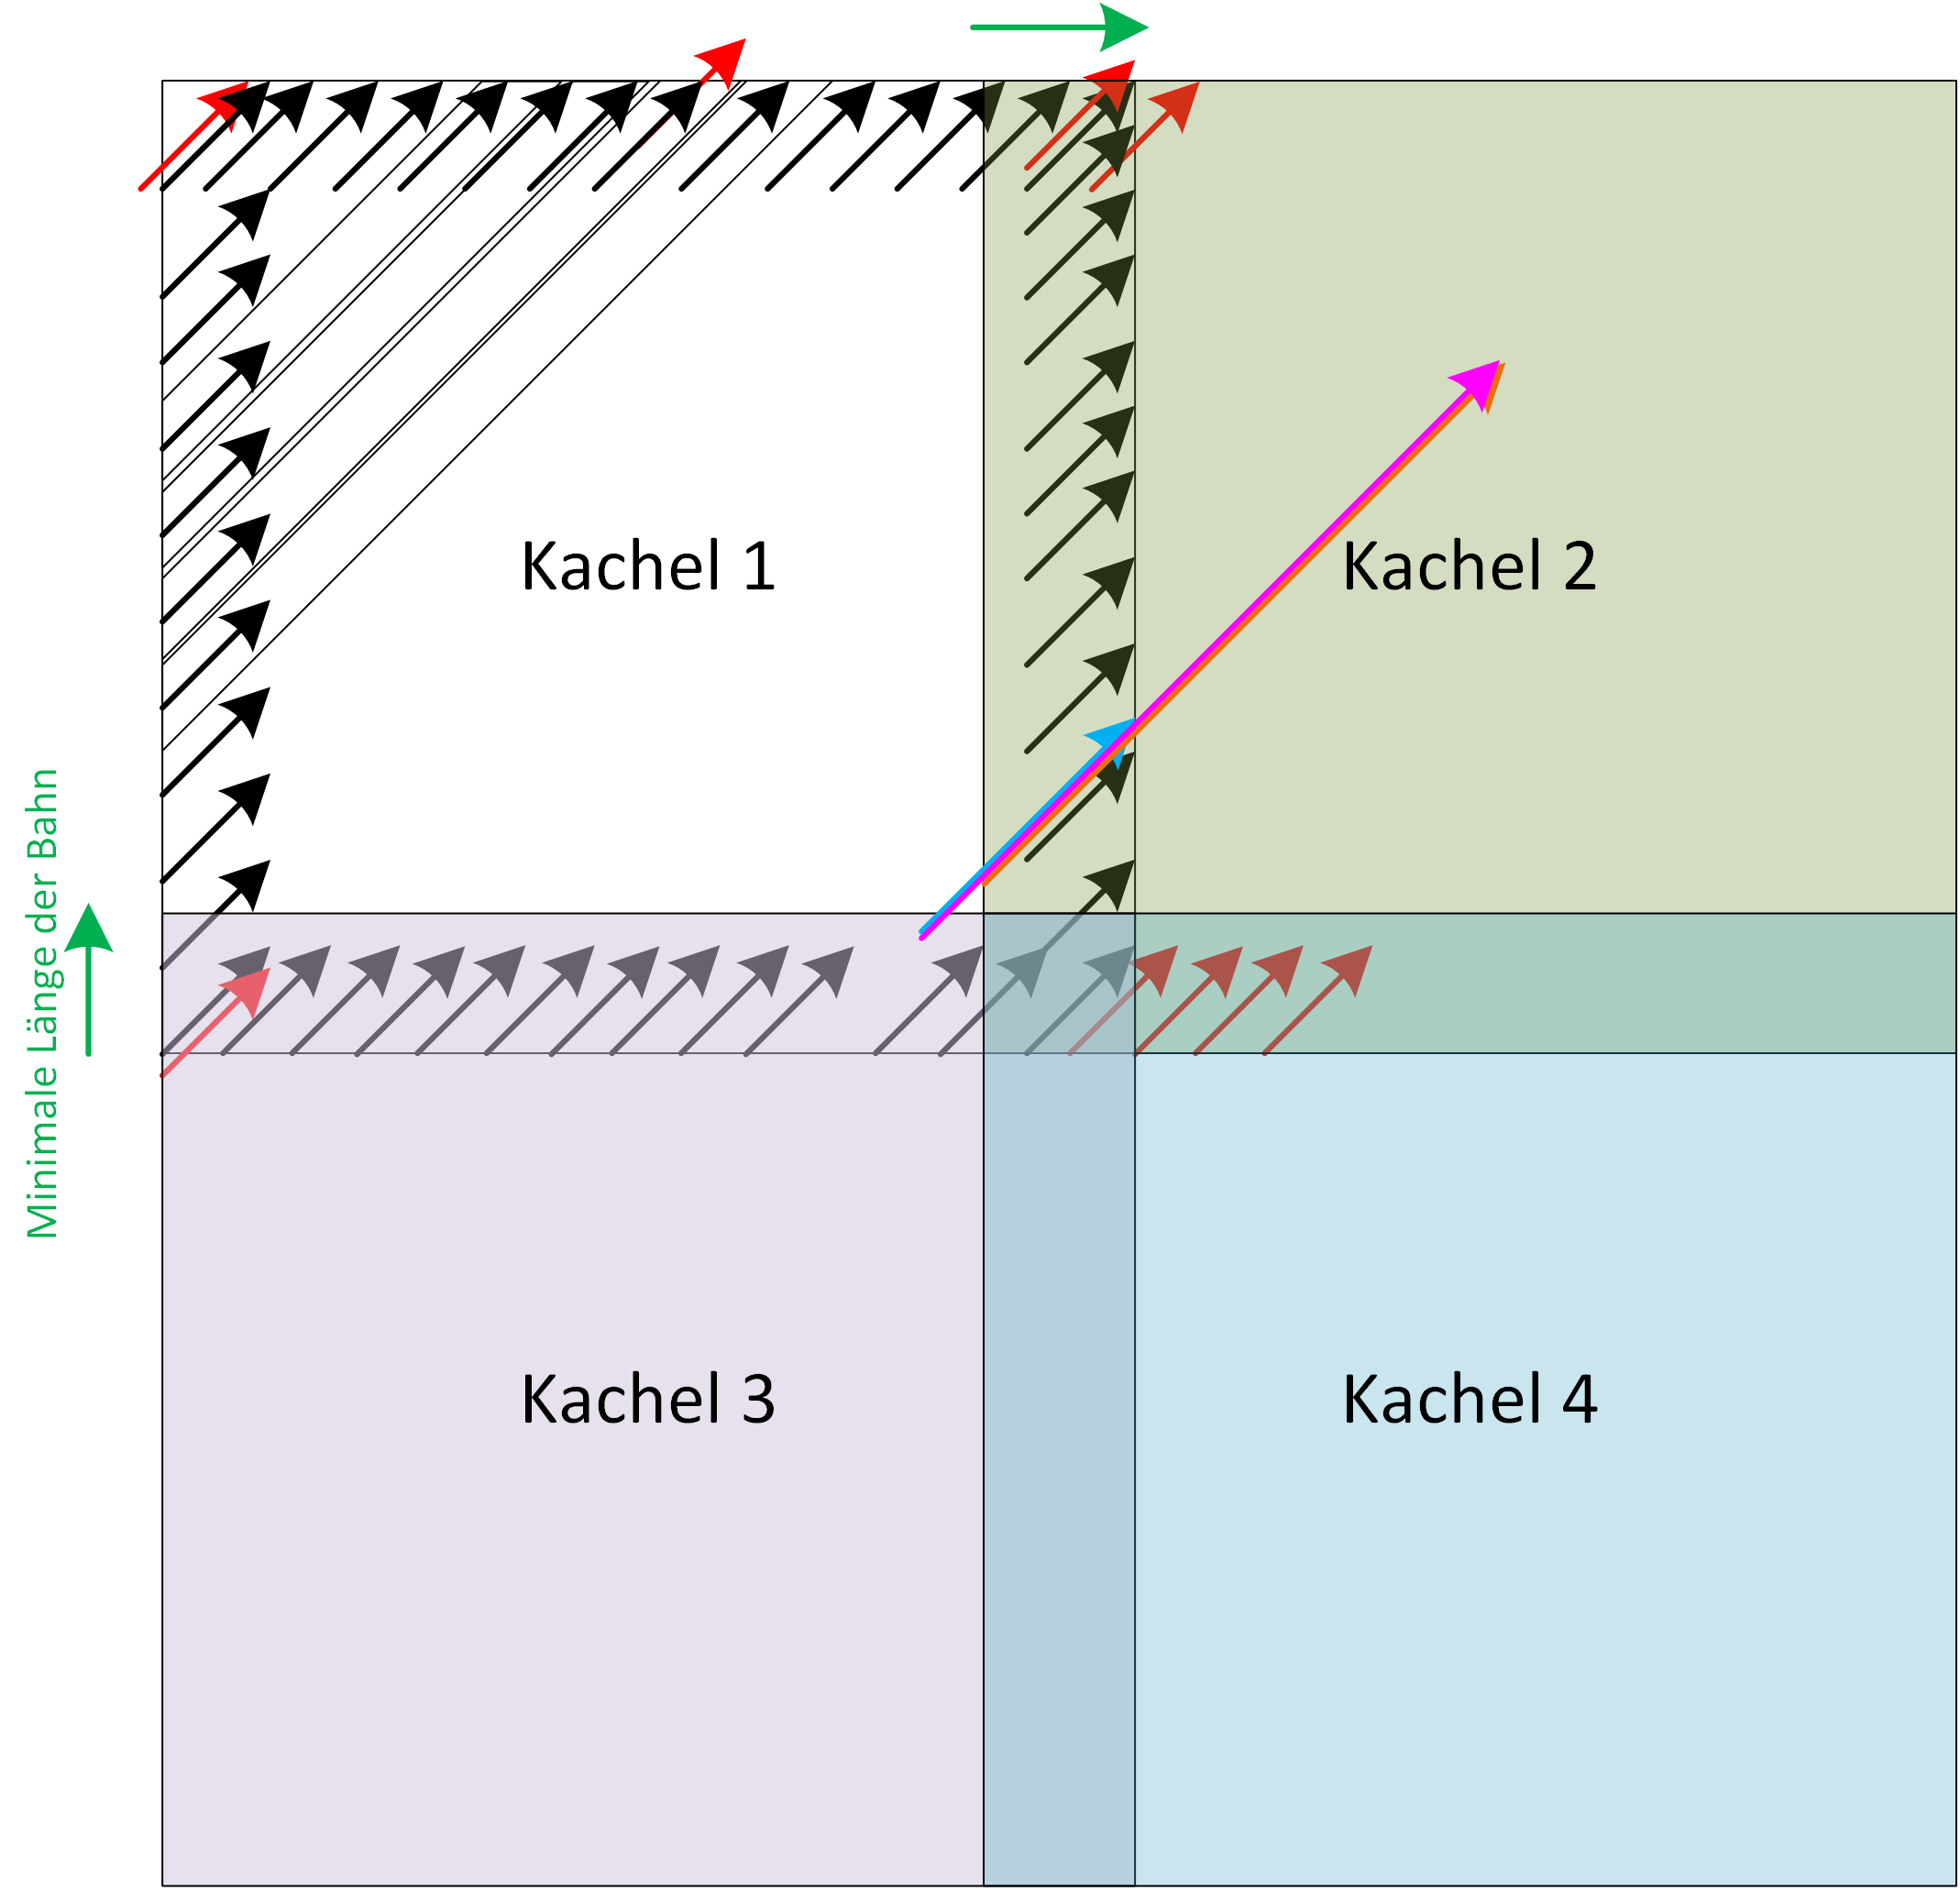
\includegraphics[width=0.5\textwidth]{../Vorgehensweise/drawings/UeberlappungKacheln.png}
	\caption{Prinzip der Kachelung bei Datensätzen, die nicht vollständig in den Speicher passen}
	\label{kachelung}
\end{figure}


In der aktuellen Implementierung ist eine künstliche Beschränkung auf die Hälfte des noch zur Verfügung stehenden RAMs eingestellt.\footnote{Der noch maximal zur Verfügung stehende Speicher lässt sich ermitteln über \texttt{size\_t maxUsableRAM = sysconf(\_SC\_AVPHYS\_PAGES) * sysconf(\_SC\_PAGESIZE);}}. Dies könnte in künftigen Versionen leicht geändert werden, war aber mit den vorhandenen Datensätzen nicht notwendig.

\subsubsection{Koordinatensysteme}

Eine große Herausforderung bei der Verarbeitung von Geodaten stellen die verwendeten Projektionen und Koordinatensysteme dar. Da es nicht möglich ist eine Kugeloberfläche (genauer eine Elipsoidoberfläche) gleichzeitig längen- und winkeltreu auf eine Ebene zu projizieren, existiert eine Vielzahl verschiedener Projektionssysteme, welche immer einen gewissen Kompromiss aus den gewählten Anforderungen darstellen. So listet allein die \href{http://geotiff.maptools.org/proj_list/}{\glqq GeoTIFF Projections Transform List\grqq} über 40 verschiedene, offensichtlich gängige Projektionen für GeoTIFF Datensätze auf.

Glücklicherweise gibt es eine sehr umfangreiche und relativ gut dokumentierte open source Bibliothek, welche die Umrechnung der verschiedenen Projektionen und Koordinatensysteme abstrahiert und zur Verfügung stellt. Diese \href{http://www.gdal.org/}{\glqq GDAL - Geospatial Data Abstraction Library\grqq} kommt auch in diesem Projekt zum Einsatz und ermöglicht es auf relativ einfache Art und Weise, die Daten aus dem GeoTIFF zu extrahieren und mit Koordinaten im WGS84-Koordinatensystem\footnote{siehe hierzu als Einstieg: \href{https://de.wikipedia.org/wiki/World_Geodetic_System_1984}{https://de.wikipedia.org/wiki/World\_Geodetic\_System\_1984}} in Einklang zu bringen. Das WGS84 System ist das aktuell in der Luftfahrt verwendete Koordinatensystem und wird auch in Navigationssystemen und insbesondere in Kartendiensten im Internet verwendet. Koordinaten im WGS84-System werden über die bekannten zwei Werte von geographischer Länge (Longitude) und geographischer Breite (Latitude) angegeben. Das Büro von Prof. Schiffmann an der Fernuniversität Hagen hat in diesem System z. B. die Koordinaten \href{http://bl.ocks.org/d/94faa16e1c8cb9d9226902f9fb0cc36c}{Lat: 51.37632449291616N, Long:7.493609189987183E}

Mit Hilfe der erwähnten Bibliothek werden innerhalb der Klasse \texttt{GeoTIFF\-Handler} Funktionen bereitgestellt, die von WGS84-Koordinaten auf Pixel im Speicher und umgekehrt umrechnen können. Damit kann die Durchmusterung auf einem reinen Pixel basierten Koordinatensystem erfolgen, während Zuordnung von Geokoordinaten vollständig aus dem Durchmusterungsprozess heraus abstrahiert ist. Es muss dem GeoTIFF-Handler lediglich am Anfang mitgeteilt werden, welcher rechteckige Ausschnitt (in Geokoordinaten) aus dem Datensatz eingelesen werden soll. Die Durchmusterung findet dann auf einem rechteckigen Pixelbereich statt. Gefundene Bahnen werden über Ihren Anfangs- und Endpunkt in Pixel-Koordinaten und ihre Breite charakterisiert und vom \texttt{GeoTIFFHandler} auf Koordinaten in WGS84 abgebildet.

\paragraph{Schwäche der vorliegenden Implementierung:} Leider hat sich zum Ende der Bearbeitungszeit herausgestellt, dass bei einem Datensatz in der Größe von NRW die zuvor getroffene Annahme falsch ist, dass das GeoTIFF-Pixel-Rechteck an jeder Stelle in Nord-Süd- bzw. Ost-West-Richtung ausgerichtet ist. In der vorliegenden Implementierung wird implizit davon ausgegangen, dass der rechte Nachbar eines jeden Pixels genau in östlicher (also 90\degree) Richtung liegt, und der untere Nachbar in südlicher (also 180\degree) Richtung. Das ist aber aufgrund der schon erwähnten Probleme mit der Projektion eines Elipsoiden auf eine Ebene nicht korrekt und so ergeben sich über die gesamte Fläche Abweichungen von wenigen Grad, wenn diese Annahme bei der Durchmusterung auf Pixel-Ebene aufrecht erhalten wird. Da es sich bei der vorliegenden Implementierung bisher noch eher um einen Proof-of-Concept handelt, wurden diese Abweichungen von der geforderten Richtung toleriert. Im Ausblick wird ein möglicher Lösungsansatz angesprochen, um dieses Problem zu lösen.


\subsubsection{Das \texttt{GeoTIFFHandler}-Objekt}

Die Search Engine hält sich während der Programmlaufzeit ein \texttt{GeoTIFFHandler}-Objekt, welches die gesamte Interaktion mit der GeoTIFF-Datei inklusive der gerade beschriebenen Transformationen übernimmt.

Dieses Objekt stellt der Suchmaschine folgende Daten zur Verfügung:

\begin{lstlisting}[language=myC]
struct datasetInfo {
	pixelPair extent = {0,0};	
		//the extent of the current dataset
	rectSize pixelSize = {0,0}; 	
		//dimension of a single pixel in [meter]
	float noDataValue = 0;	//marker for "no data" in the dataset;
		//the marker value for invalid/non existant pixels
};	
\end{lstlisting}

Dies sind die für die Durchmusterung relevanten globalen Daten über den Datensatz. Die Koordinaten der Eckpunkte können über die Funktion \\
\verb|geoCoord pixel2Geo(const pixelCoordFloat source);| abgefragt werden, falls das nötig ist. Wesentlich ist vor allem die Angabe des "`ungültig Werts"' innerhalb der Pixel im Speicher.

Sobald der Benutzer eine Auswahl getroffen hat, welchen Bereich der Welt er nach Notlandefeldern durchmustern möchte, kann über den Aufruf der Funktion 
\begin{lstlisting}[language=myC]
resultType getTilingInfo(const geoCoord topLeft, const geoCoord bottomRight, const float overlap, const size_t maxSize, tilingCharacteristics *tilingResult);
\end{lstlisting}

das \texttt{GeoTIFFHandler}-Objekt angewiesen werden, das Einlesen der Daten in den Speicher vorzubereiten und Informationen darüber bereitzustellen, ob die Daten eventuell in mehreren Kacheln verarbeitet werden müssen. Dazu wird eine spezielle Datenstruktur gefüllt:
\begin{lstlisting}[language=myC]
struct tilingCharacteristics {
	int overallXSize = 0, overallYSize = 0;	
		//the extent of the currently requested cutout of the dataset
	pixelCoord topLeftPix = {0,0};	
		//top left pixel coordinate of the requested area
	pixelCoord bottomRightPix = {0,0};	
		//bottom right pixel coordinate of the requested area
	int maxTileSizeXPix = 0, maxTileSizeYPix = 0;
	int overlapXPix =0, overlapYPix =0;
	int tilesInX = 0, tilesInY = 0;	
		//the amount of tiles in X- and Y-direction
	float overlap = 0;	
		//the overlap of the tiles in [meter]
	size_t maxTileMemsize = 0;	
		//the maximum amount of bytes a tile needs in memory
};
\end{lstlisting}

Diese Angaben sind ausreichend, um die Durchmusterung auf Pixelebene zu beginnen. Das \texttt{GeoTIFFHandler}-Objekt kann angewiesen werden, nacheinander die einzelnen Kacheln (oder auch nur die eine Kachel) in den Speicher zu laden, so dass sie durchsucht werden können. Die gesamte Speicherverwaltung wird durch den \texttt{GeoTIFFHandler} übernommen, weswegen vor dem Laden der nächsten Kachel auch die aktuell verwendete Kachel explizit wieder freigegeben werden muss.

Zusätzlich werden noch einige Datenstrukturen und Hilfsfunktionen zur Verfügung gestellt, die (hoffentlich einigermaßen) selbsterklärend sind.
Die wesentlichen zur Verfügung gestellten Funktionen sind:
\begin{lstlisting}[language=myC]
	resultType getDatasetInfo(datasetInfo *info);
	resultType getPixelExtent(rectSize *pixelSize);
	resultType getTilingInfo(const geoCoord topLeft, const geoCoord bottomRight, const float overlap, const size_t maxSize, tilingCharacteristics *tilingResult);
	resultType getTile(const int xTile, const int yTile, tileData *tile);
	resultType releaseTile(const int xTile, const int yTile);

	geoCoord pixel2Geo(const pixelCoordFloat source);
	geoCoord pixel2Geo(const int xTile, const int yTile, const pixelCoordFloat source);
	pixelCoord geo2Pixel(const geoCoord source);
	pixelCoord geo2Pixel(const int xTile, const int yTile, const geoCoord source);

	/**
	 * returns a valid geoJSON Object with empty properties
	 * These have to be overwritten later on.
	 * see https://gis.stackexchange.com/questions/144084/using-gdal-c-to-calculate-distance-in-meters
	 * see https://geographiclib.sourceforge.io/1.40/C/inverse_8c_source.html
	 */
	json getGeoJsonPolygon(const pixelCoordFloat start, const pixelCoordFloat end, const float width);
	json getGeoJsonPolygon(const pixelCoordFloat start, const float length, const float heading, const float width);
	json getGeoJsonPolygon(const pixelCoordFloat pix0, const pixelCoordFloat pix1, const pixelCoordFloat pix2, const pixelCoordFloat pix3);
\end{lstlisting}

\section{Komponente "'Durchmusterung"'}
\subsection{Durchmusterung der Geotiff Daten und Auffinden der Landebahnen}
Die Durchmusterung der Geodaten wurden in einer eigenen statischen Library gekapselt (\texttt{plane\_library.a}). Innerhalb dieser Library finden sich alle Algorithmen, die zum Auffinden der Landebahnen benötigt werden. Für den Aufrufer ist die Implementation komplett gekapselt. Alle funktionalen Requirements werden von dieser Library übernommen.


\subsection{Interface der Library}

Die Parameter des Interfaces sind im Listing \ref{interface} beschrieben.

\begin{lstlisting}[language=myC, caption=Interface Beschreibung, label=interface]
int search_for_planes(const tileData *actualTile, GeoTiffHandler *myGeoTiffHandler, float heading, float minLength, float width, int commSocket, const json *taskDescription, float noDataValue , rectSize pixelSize );
\end{lstlisting}

Die einzelnen Aufrufparameter und deren funktionale Eigenschaft sind in Tabelle~\ref{beschreibungparameter} aufgezeigt.

\begin{table}[htb]
\centering
\begin{tabular}{|p{4.5cm}|p{10cm}|}
\hline 
\bf{Parameter} & \bf{Funktion} \\ 
\hline 
*actualTile & Zeiger auf das Geo-Kartenobjekt mit den individuellen Höhendaten \\ 
\hline 
*myGeoTiffHandler & Zeiger auf eine Instanz eines GeoTiffHandler Objekts, 
welches diverse Funktionen zur Umrechnung, Konvertierung etc. im GeoTiff Format unterstützt \\ 
\hline 
heading & Durchmusterungswinkel für die Landebahnen $0^\circ =>$ Süd-Nord Achse \\ 
\hline 
minLength & minimale geforderte Länge der Landebahn in [m] \\ 
\hline 
width & Breite der geforderten Landebahn in [m] \\ 
\hline 
commSocket & Unix-Socket zur Kommunikation mit dem Database Manager zum Abspeichern gefundener Landebahnen\\ 
\hline 
*taskDescription & Taskbeschreibung, die vom Database Manager geliefert wurde\\ 
\hline 
noDataValue & Zahlenwert für undefinierte Kartenpunkte \\ 
\hline 
pixelSize & Auflösung der Rasterpunkte in [m]\\
\hline 

\end{tabular} 
\caption{Beschreibung der Aufrufparameter Funktionalität}\label{beschreibungparameter}
\end{table}

\subsection{Logischer Ablauf innerhalb der Landebahn-Erkennung}

Der logische Ablauf ist schematisch im Nassi-Shneiderman-Diagramm~\ref{nasshnlogisch} dargestellt.

\clearpage
\begin{figure}
\begin{struktogramm}(100,200)
  \assign{Initialisierung $tile\_worker$ Objekt}
  \assign{berechne winkel-, steigungs- und holprigkeitsabhängige Parameter}
\forallin{für alle Startpunkte einer Landebahn in gegebener Richtung (Thread Pool)}
\assign{wähle den nächsten Punkt}
\ifthenelse[15]{1}{1}
{kurzreichweitige Steigung zum Vorgänger OK?}{\sTrue}{\sFalse}
\ifthenelse[17]{1}{6}
{checke Holprigkeit in Querrichtung}{\sTrue}{\sFalse}
\change
\ifthenelse[40]{1}{1}
{ist die aktuelle Landebahn länger als die Mindestlänge}{\sTrue}{\sFalse}
\assign{suche die beste Landebahn mit Mindestlänge}
\assign{speichere beide Landebahnen in der DB}
\assign{starte eine neue Landebahn mit aktuellem Punkt}
\change
\assign{starte eine neue Landebahn mit aktuellem Punkt}
\ifend
\ifend
\change
\ifthenelse[30]{1}{1}
{ist die aktuelle Landebahn länger als die Mindestlänge}{\sTrue}{\sFalse}
\assign{suche die beste Landebahn mit Mindestlänge}
\assign{speichere beide Landebahnen in der DB}
\assign{starte eine neue Landebahn mit aktuellem Punkt}
\change
\assign{starte eine neue Landebahn mit aktuellem Punkt}
\ifend
\assign{starte eine neue Landebahn mit aktuellem Punkt}
\ifend
\forallinend
\end{struktogramm}
\caption{Durchmusterungsalgorithmus in Pseudo-Code}
\label{nasshnlogisch}
\end{figure}
\clearpage
\subsection{Initialisierung}

Die Initialisierung erzeugt zunächst ein \texttt{tile\_worker} Objekt und initialisiert die Instanzvariablen mit den bei der Objekterzeugung angegebenen Durchmusterungscharakteristika wie maximal erlaubte Steigung, Varianz und minimale Landebahnlänge.
Mit dem Aufruf von \texttt{check\_steigungen()} werden dann die optimalen Schrittvektoren und die Startkoordinaten des Durchmusterungsvorgangs bestimmt.

Die optimalen Durchmusterungsvektoren sind winkelabhängig. Die Idee hierbei ist, dass in Abhängigkeit der Auflösung diese Vektoren so initialisiert werden, dass alle möglichen Landebahnen gefunden werden. Dies führt dazu, dass bestimmte Winkel beim Durchmustern dichtere Landebahnen abtasten können. Somit wird sichergestellt, dass jede Landebahn mindestens einmal untersucht wird.
Zusätzlich dazu werden dann orthogonale Vektoren aus den Schrittvektoren abgeleitet, die zum Durchmustern in orthogonaler Richtung (Landebahnbreite) benutzt werden.

Anhand der gegebenen Kartenauflösung und Schrittvektoren kann im Anschluss bestimmt werden, wie viele aufeinander folgende Punkte mindestens benötigt werden, damit die Landebahn die Mindestlängenvoraussetzung erfüllt.
Entsprechendes gilt natürlich auch für die Breite der Bahn.

Anschließend werden die Startpunkte der Durchmusterung bestimmt.
Diese sind abhängig vom Durchmusterungswinkel. 
Für Winkel, die ein Vielfaches von 90 betragen, wird einfach eine Seite des Quadranten abgeschritten. Wird eine Bahn z. B. in $y$-Richtung abgetastet, wird der Abszissenwert inkrementiert / dekrementiert und erneut in $y$-Richtung abgeschritten, bis der Rand der Kachel erreicht wird. Eine schematische Darstellung findet sich in Abbildung~\ref{scanortho}.

Bei Winkeln, die nicht einem Vielfachen von 90 entsprechen, werden sukzessiv sowohl Abszisse als auch Ordinate abgeschritten und das Terrain in Diagonaler Richtung durchmustert. 
Eine schematische Abbildung hierzu findet sich in Abbildung~\ref{scandiagonal}. Hier wird zunächst die Abszisse bis zum Ursprung abgeschritten, bevor der Ordinatenwert inkrementiert wird.

\begin{figure}
\centering
\begin{tikzpicture}
\draw[help lines, color=gray!30, dashed] (0,0) grid (4.9,4.9);
\draw[->,ultra thick] (0,5)--(5,5) node[right]{$x$};
\draw[->,ultra thick] (0,5)--(0,0) node[left]{$y$};

\draw[-,ultra thick] (5,5)--(5,0) node[left]{};
\draw[-,ultra thick] (0,0)--(5,0) node[right]{};

\draw[->,ultra thick,dashed,red] (4,5)--(5,4) node[left]{$1$};
\draw[->,ultra thick,dashed,red] (3,5)--(5,3) node[left]{$2$};
\draw[->,ultra thick,dashed,red] (0,5)--(5,0) node[right]{$3$};

\draw[->,ultra thick,dashed,red] (0,3)--(3,0) node[below]{$4$};

\draw[->,ultra thick,dashed,red] (0,1)--(1,0) node[below]{$5$};

\draw[-,ultra thick,dashed,blue] (5,5.5)--(-0.5,5.5) node[left]{};
\draw[->,ultra thick,dashed,blue] (-0.5,5.5)--(-0.5,0) node[left]{};
\end{tikzpicture}
\caption{Verschiebung des Startpunkts der Landebahndurchmusterung in diagonaler Richtung. Hier NNO nach SSW. Der Startpunkt der einzelnen Bahnen folgt dem blauen Pfeil.}
\label{scandiagonal}
\end{figure}


\begin{figure}
\centering
\begin{tikzpicture}
\draw[help lines, color=gray!30, dashed] (0,0) grid (4.9,4.9);
\draw[->,ultra thick] (0,5)--(5,5) node[right]{$x$};
\draw[->,ultra thick] (0,5)--(0,0) node[left]{$y$};

\draw[-,ultra thick] (5,5)--(5,0) node[left]{};
\draw[-,ultra thick] (0,0)--(5,0) node[right]{};

\draw[->,ultra thick,dashed,red] (0,5)--(0,0) node[below]{$1$};
\draw[->,ultra thick,dashed,red] (1,5)--(1,0) node[below]{$2$};
\draw[->,ultra thick,dashed,red] (3,5)--(3,0) node[below]{$3$};
\draw[->,ultra thick,dashed,red] (5,5)--(5,0) node[below]{$4$};


\draw[->,ultra thick,dashed,blue] (-0,5.5)--(5,5.5) node[left]{};
\end{tikzpicture}
\caption{Verschiebung des Startpunkts der Landebahndurchmusterung in diagonaler Richtung. Hier N nach S. Der Startpunkt der einzelnen Bahnen folgt dem blauen Pfeil.}
\label{scanortho}
\end{figure}
\subsection{Parallelverarbeitung mittels p\_threads zum Finden der Landebahnen}

Die Parallelverarbeitung arbeitet nach einem Task-Workermodell, welches mit einem Semaphor gesteuert wird. Jeder Startpunkt, der auf einem Kartenrand liegt, ist hier als ein Task anzusehen. Das Semaphor dient dazu, die gleichzeitige Anzahl der Threads zu steuern und zu kontrollieren. Dies dient zum einen Untersuchungszwecken, um festzustellen, wie der Speedup bei Variation der Threads ist. Weiterhin würde eine zu hohe Zahl an an Threads die ausführende Maschine in extreme Ressourcenknappheit bringen können.

Das Workerobjekt kontrolliert mit einem \texttt{mutex} die Herausgabe von Startwerten. In einem kritischen Bereich wird durch Inkrementierung des Startpunktes ein neuer Startpunkt generiert, der an einen Worker als Form eines abzuarbeitenden Task herausgegeben wird. Dieser kritische Bereich, der dafür sorgt, dass jeder Startpunkt auch nur wirklich einmal herausgeben wird, stellt somit auch das Bottleneck der Parallelverarbeitung dar. So lange die Anzahl der Punkte pro Bahn und die Berechnungszeit, die ein Thread benötigt, um die Bahn in der vorgegebenen Richtung abzuscannen und die zur Bahn gehörigen Parameter wie Varianz etc. zu berechnen größer ist als die Zeit, die vergeht, bis der Thread wieder in der Warteschlange zum Erhalt eines neuen Startwertes aufläuft, sollte dieses Bottleneck gering sein.

Zudem ist zu beachten, dass natürlich nicht alle Landebahnen gleich lang sind. So lange der Startpunkt in der Nähe einer Kartenecke ist und die Durchmusterungsrichtung nur wenige Punkte bis zum Kartenrand umfasst, wird die Durchmusterung schnell vorbei sein und ein neuer Startwert benötigt werden. Dies wird in Abbildung~\ref{scandiagonal} deutlich. Mit der potentiellen Landebahn 3 hat der Thread die meisten Punkte abzuarbeiten während die Bahnen 1 und 5 relativ schnell abgearbeitet sein werden. 

\subsection{Detaillierte Beschreibung des Suchalgorithmus}

Ausgehend vom jeweiligen Startpunkt wird mittels \texttt{p\_thread\_create} ein neuer Thread erzeugt und die Funktion \texttt{void *thread\_data::check\_single\_plane (void *x\_void\_ptr)} als Startroutine mitgegeben. Innerhalb dieses erzeugten Threads existiert eine while Schleife, die solange true returniert, wie noch nicht alle Startpunkte an Threads ausgeben wurden.

Innerhalb einiger verschachtelter Bedingungen wird überprüft, ob der betrachtete Geopunkt tatsächlich Höheninformationen hat und ob die Steigung zu seinem unmittelbaren Vorgänger innerhalb des erlaubten Bereiches liegt.

Trifft dies zu, so ist noch die Steigung benachbarter Punkte in orthogonaler Richtung zu betrachten. Sind all diese Kriterien erfüllt, wird der betrachtete Geopunkt in eine Liste gültiger Punkte aufgenommen. Diese Prozedur wird so lange wiederholt, bis ein Kriterium nicht mehr erfüllt oder der Kartenrand erreicht ist.

Ist eines dieser Abbruchkriterien erfüllt, wird überprüft, ob das Ensemble aneinanderhängender Punkte die Mindestlänge der geforderten Landebahn erfüllt.

Dann wird eine Subroutine \texttt{find\_best\_planes()} aufgerufen, welche innerhalb der gefunden Liste zusammenhängender Punkte zwei Landebahnen ermittelt. Zum einen wird die längste Bahn, die das Steigungskriterium erfüllt ermittelt und zum Anderen die Landebahn, welche die geringste Varianz aufweist und trotzdem noch die geforderte Mindestlänge erreicht. 
Beide Bahnen werden an den Database Manager übermittelt.

\subsection{Klassen und Objekte}

In der \texttt{plane\_library.a} werden mehrere Klassenimplementationen verwendet, um objektorientiert zu einer vereinfachten Problemlösung zu gelangen.

Die zentrale Klasse ist dabei die \texttt{tile\_worker}-Klasse. In ihr werden wichtige Membervariablen zu den parametrisierten Rahmenbedingungen verwaltet und das Threading mittels p\_thread abgehandelt. Die Klasse \texttt{landing\_plane} beschreibt ein Hilfsobjekt, in dem gefundene Landebahnobjekte via Startpunkten, Steigung und Varianz beschrieben wird.
Das Threading selbst hat eine sehr schlanke \texttt{thread\_data}-Klasse, welche in einer \glqq friend\grqq -Beziehung zum \texttt{tile\_worker} steht und sich ausschließlich mit der Parallelausführung beschäftigt.

Der \texttt{tile\_manager} ist eine Klasse, die ausschließlich zu Debug- und Entwicklungszwecken zum Bau eines Standalone Binaries benötigt wird.
Für den produktiven Einsatz ist sie obsolet.


\subsection{Verwendete Datenstrukturen}

Die wichtigsten Datenstrukturen, die während der Durchmusterung benötigt werden, sind das übergebene Kachelobjekt, ein Objekt zur Verwaltung der aktuell gefundenen zusammenhängenden Punkte, sowie der \texttt{tile\_worker}, der die Threads kontrolliert und Durchmusterungsparameter kapselt. 

\subsubsection{Einfluss der Datenstrukturen auf die Performanz}

Die Container-Klasse des \texttt{tile\_worker} hat in ihrer endgültigen Form keine komplexeren Datenstrukturen mehr. Sie beinhaltet lediglich Membervariablen einfacher Datentypen wie \texttt{double} und \texttt{int}.

Innerhalb der Thread-Klasse findet sich eine lokale Variable \texttt{coordlist}, welche vom Typ \texttt{vector< pair<int,int> >} ist.
Hier werden temporär aneinanderhängende Ketten von Landebahnpunktkoordinaten vorgehalten. Die gespeicherten Punkte sind dabei lediglich Referenzen auf das statische Kartenobjekt. Ohne dieses wären die Informationen bedeutungslos.

Der Vorteil des vector templates in C++ ist der optimierte random access, welcher in der Komplexizitätsklasse $\mathcal O(1)$ einzugruppieren ist und die Verwaltung sehr komfortabel mittels Member-Funktionen bereitstellt.

Das Kachelobjekt selbst stellt die Höheninformationen eines 2-dimensionalen Kartenausschnitts in einem linearen Array dar. Der Durchmusterungsalgorithmus benötigt allerdings einen Mappingmechanisumus eines 2-dimensionalen Punktes auf das eindimensionale Array.

Dies wird von der Funktion \texttt{access\_single\_element(int\ x, int\ y)} bereitgestellt. Anhand der Information, wie viele Datenpunkte der Kartenausschnitt in $x$-Richtung beinhaltet, wird das Mapping auf das eindimensionale Array dargestellt. Im Falle einer Bereichsüberschreitung, wird \texttt{numeric\_limits <float>::min()} zurückgegeben.
Auch dieser Zugriff ist der Komplexitätsklasse $\mathcal O(1)$ zuzuordnen und unabhängig von der Datengröße.

\begin{lstlisting}[language=myC]
float tile_worker::access_single_element(int x, int y)
{
  if (tile->width.x*y+x < tile->width.x*tile->width.y)
    return(tile->buf[tile->width.x*y+x]);
  else
   return numeric_limits<float>::min();
}
\end{lstlisting}

Dies führt dazu, dass der Speicherbedarf ausschließlich von der Anzahl der Datenpunkte in den Rohdaten abhängig ist. Für die Speicherallokierung werden insbesondere bei den C++ Templates vordefinierte default-Allokatoren genutzt, die man natürlich mit eigens definierten überladen könnte. Dafür gibt es bislang aber keinerlei Notwendigkeit.
 


\subsection{Bestimmung des Speedups in Abhängigkeit des Parallelisierungsgrades}

Um den Speedup zu bestimmen, wurde analysiert, wie sich die Laufzeit mit zunehmender Anzahl an Threads verändert. So lange die Bearbeitung einer einzelnen Bahn viel länger dauert als die in der kritischen Sektion benötigte Zeit, um einen neuen Startpunkt zu bestimmen, sollten die Threads nicht blockiert sein.

Bei Winkeln, die ein Vielfaches von $90$ betragen, sind alle Landebahnen gleich lang --- also sind gleich viele Punkte zu analysieren (siehe Abbildung~\ref{scanortho}).

Bei Bahnen, die diagonal verlaufen, sind die ersten Bahnen kurz, nehmen dann in ihrer Länge zu, bis als Startpunkt die nächstliegende Ecke erreicht ist, und nehmen dann in ihrer Länge wieder ab (siehe Abbildung~\ref{scandiagonal}). 
Weiterhin ist zu beachten, dass je nach Topologie der Bahn unterschiedlich viele (im Grenzfall gar keine) geeignete Flächen gefunden werden, die dann fein granular weiter untersucht werden müssen (längste Bahn und die mit der kleinsten Varianz). So ist schwer vorhersagbar, wie lange die Einzellaufzeit eines Threads ist.
Für die zur Verfügung gestellten Kartendaten von Nordrhein-Westfalen sind die Laufzeiten in Abhängigkeit von Winkel und Threadanzahl in Tabelle~\ref{laufzeiten} dargestellt.

\subsubsection{Erläuterung des Messverfahren}

Die Messung wurde in einer virtualisierten Umgebung durchgeführt. Als Host-System diente ein Windows 7 64 bit System, welches hardwaretechnisch auf einem Intel i7-4770K , 3.5 Ghz, 16 GB RAM System lokalisiert ist. Die Virtualisierung wurde mit Virtualbox mit einem Linux Guest System (Centos Linux 7.0, 6 GB RAM) durchgeführt. 
Die Anzahl der virtuellen CPUs wurde von 1-8 variiert.
Pro vorgegebener Parametrisierung wurden 4 unabhängige identische Messungen gemacht. In Tabelle~\ref{laufzeiten} angegeben ist der Mittelwert mit Standardabweichung dieser Läufe.
 

\subsubsection{Messergebnisse}
\begin{figure} 
\begin{tabular}{|c|c|c|c|c|c|}
\hline 
Richtung & Bahnen & Threads & v CPUs & Zeitbedarf [ms] & Standardabweichung [ms] \\ 
\hline 
N$\rightarrow$S (0$^\circ$) & 734 & 1 & 1 & 11409 & 510 \\ 
\hline 
N$\rightarrow$S (0$^\circ$) & 734 & 2 & 1 & 11049& 216 \\ 
\hline 
N$\rightarrow$S (0$^\circ$) & 734 & 4 & 1 & 11586 & 220 \\ 
\hline 
N$\rightarrow$S (0$^\circ$) & 734 & 8 & 1 & 11230 & 240 \\ 
\hline 
N$\rightarrow$S (0$^\circ$) & 734 & 64 & 1 & 10886 & 621 \\ 
\hline 
W$\rightarrow$O (90$^\circ$) & 1606 & 1 & 1 & 10442 & 239 \\ 
\hline 
W$\rightarrow$O (90$^\circ$) & 1606 & 64 & 1 & 10094 & 284 \\ 
\hline 
NNO$\rightarrow$SSW (45$^\circ$) & 704 & 1 & 1 & 18147 & 327 \\ 
\hline 
NNO$\rightarrow$SSW (45$^\circ$) & 704 & 64 & 1 & 18423 & 701 \\ 
\hline 
N$\rightarrow$S (0$^\circ$) & 734 & 1 & 2 & 8488 & 46 \\ 
\hline 
N$\rightarrow$S (0$^\circ$) & 734 & 2 & 2 & 5397 & 178 \\ 
\hline 
N$\rightarrow$S (0$^\circ$) & 734 & 4 & 2 & 5545 & 161 \\ 
\hline 
W$\rightarrow$O (90$^\circ$) & 1606 & 1 & 2 & 8668 & 453 \\ 
\hline 
W$\rightarrow$O (90$^\circ$) & 1606 & 2 & 2 & 5778 & 292 \\ 
\hline 
NNO$\rightarrow$SSW (45$^\circ$) & 704 & 1 & 2 & 15208 & 216 \\ 
\hline 
NNO$\rightarrow$SSW (45$^\circ$) & 704 & 64 & 2 & 8976 & 327 \\ 
\hline
N$\rightarrow$S (0$^\circ$) & 734 & 1 & 4 & 8823 & 83 \\ 
\hline 
N$\rightarrow$S (0$^\circ$) & 734 & 2 & 4 & 4642 & 77 \\ 
\hline 
N$\rightarrow$S (0$^\circ$) & 734 & 4 & 4 & 2973 & 17 \\ 
\hline 
N$\rightarrow$S (0$^\circ$) & 734 & 8 & 4 & 3571 & 432 \\ 
\hline 
W$\rightarrow$O (90$^\circ$) & 1606 & 8 & 4 & 3335 & 72 \\ 
\hline 
NNO$\rightarrow$SSW (45$^\circ$) & 704 & 8 & 4 & 5406 & 442 \\ 
\hline
N$\rightarrow$S (0$^\circ$) & 734 & 16 & 8 & 2733 & 56 \\ 
\hline 
\end{tabular}
\caption{Laufzeiten verschiedener Durchmusterungen in Abhängigkeit der Threads und virtuellen CPUs}\label{laufzeiten}
\end{figure} 

\subsubsection{Diskussion der Messergebnisse}

Als Landebahneigenschaften wurden eine Länge von 4000~m, eine Holprigkeit in Längs- und Querrichtung von 3~\%, sowie eine maximale Steigung von 10~\% gefordert. Dieses Parameterset wurde so gewählt, dass nicht zu viele Landebahnen in die Datenbank geschrieben werden müssen, da dies auch einen signifikanten CPU Anteil benötigt. Weiterhin ist das Rendering im Browser bei sehr vielen Bahnen CPU-intensiv. Daher erschien das oben gewählte Parameterset als schlüssig.
Auffällig ist, dass selbst im Singlethreadbetrieb bei der Erhöhung der CPUs ein Speedup entsteht. Dies ist dem Umstand geschuldet, dass auf derselben VM noch der Browser und die Datenbankengine gehostet sind.
Trotzdem wird das Parameterset 1 CPU, 1 Thread als Referenz für den Speedup betrachtet.

\begin{figure}
\begin{tabular}{|c|c|}
 \hline 
 Anzahl CPU & Speedup \\ 
 \hline 
 1 & 1 \\ 
 \hline 
 2 & 2,11 \\ 
 \hline 
 4 & 3,84 \\ 
 \hline 
  8 & 4,2 \\ 
 \hline 
 \end{tabular}  
 \caption{Speedup am Beispiel der Messergebnisse in Nord- / Südausrichtung.}
\end{figure}

\begin{figure}
\begin{tabular}{|c|c|}
 \hline 
 Anzahl CPU & Speedup \\ 
 \hline 
 1 & 1 \\ 
 \hline 
 2 & 1,8 \\ 
 \hline 
 4 & 3,13 \\ 
 \hline 
 \end{tabular}  
 \caption{Speedup am Beispiel der Messergebnisse in Ost- / Westausrichtung.}
\end{figure}

\begin{figure}
\begin{tabular}{|c|c|}
 \hline 
 Anzahl CPU & Speedup \\ 
 \hline 
 1 & 1 \\ 
 \hline 
 2 & 2,02 \\ 
 \hline 
 4 & 3,35 \\ 
 \hline 
 \end{tabular}  
 \caption{Speedup am Beispiel der Messergebnisse in Nordnordwest- / Südsüdostausrichtung.}
\end{figure}

Weiterhin zeigt sich, dass eine weitere Erhöhung der Threadanzahl über die tatsächlich verfügbaren CPUs ab einem gewissen Punkt schädlich ist.
Im Falle von 8 CPUs sind die Ergebnisse unter Umständen nicht aussagekräftig, da die Virtualisierungssoftware eine ungültige Konfiguration anzeigte. Zudem braucht auch das Host Betriebssystem Ressourcen, die natürlich nicht der VM und der Software zur Verfügung stehen.

\begin{tikzpicture} 
\begin{axis}[ 
  xlabel=Anzahl CPU, ylabel=Speedup, legend style={at={(axis cs:8.3,1)},anchor=south east}] 
  \addplot[color=red,mark=x] coordinates { 
  (1,1) 
  (2,2.11) 
  (4,3.84) 
  (8,4.2)   
  }; 
    \addplot[color=blue,mark=x] coordinates { 
  (1,1) 
  (2,1.8) 
  (4,3.13)    
  }; 
    \addplot[color=green,mark=x] coordinates { 
  (1,1) 
  (2,2.02) 
  (4,3.35)    
  }; 
    \addlegendentry{Nord-Süd}
  \addlegendentry{Ost-West}
    \addlegendentry{Nordnordwest-Südsüdost}
  \end{axis} 

  \end{tikzpicture}
  
Eine weiterführende Analyse war aufgrund mangelnder Hardwareressourcen nicht möglich.


\subsection{Analyse mittels Profiler}

Mittels gproof wurde analysiert, welche Programmteile beim Auffinden der Landebahn die meiste Rechenzeit benötigen. Hierdurch kann kontrolliert werden, ob die vom Scheduler zur Verfügung gestellten Zeitscheiben auch effektiv innerhalb des Threadings genutzt werden können. 

Bei der Analyse zeigt sich, dass die Funktion, die die meiste Zeit in Anspruch nimmt, die Zugriffsfunktion auf die Geopunkte ist. Hier findet ein Random Memory access statt (2-Dimensionalität wird auf ein eindimensionales Array abgebildet).
Eine weitere zeitintensive Funktion stellt die Berechnung der Varianz sowie das Auffinden der längsten und der varianzminimalen Landebahn dar.

Diese Ergebnisse sind intuitiv zu erwarten.
Da beide Funktionen innerhalb des Threading aufgerufen werden, ist aus laufzeittechnischer Sicht eine optimale Lösung gefunden. 

\subsection{Einfluss von Compiler Direktiven (speziell Optimizer)}

Bevor Codeausführung mittels Parallelverarbeitung zur Beschleunigung gebracht werden soll, lohnt es sich meist, durch geeignete Compilerdirektiven die serielle Codeausführung zu beschleunigen.

Der Code wurde mit einem gcc Version 4.8.5 devtoolset version 4 compiliert. Per default findet dabei eine Übersetzung ohne eingeschalteten Optimizer statt. 
Durch die Benutzung des -O3 Optimizer Direktivs ist eine Codebeschleunigung von 1300~\% (11 sec vs. 147 sec) beobachtet worden. 
Eine Übersicht über die verwendeten Optimierungsschritte sind unter \footnote{\url{https://gcc.gnu.org/onlinedocs/gcc/Optimize-Options.html}} einzusehen.

\section{Komponente "`databaseManager"'}

Im Architekturüberblick in Abbildung \ref{architektur} ist zu erkennen, dass in der Komponente \texttt{databaseManager} die gesamte Kommunikation der anderen Komponenten zusammen läuft. Tatsächlich ist diese Komponente die zentrale Schaltstelle, von der aus alle anderen Programmteile aufgerufen und gesteuert werden. Sie stellt in einer an MVC angelehnten Architektur den Controller dar.

Um diese Aufgabe zu erfüllen muss der Database Manager mehrere Interfaces zur Verfügung stellen:
\begin{itemize}
	\item eine Verbindung über UNIX-Sockets zur Search Engine
	\item eine REST-API zur Kommunikation mit dem User Interface, also dem Benutzer
	\item eine Schnittstelle zur Datenbank
\end{itemize}

Der Database Manager wurde als JavaScript Applikation in der serverseitigen Laufzeitumgebung Node.js\footnote{siehe dazu: \href{https://nodejs.org/en/}{https://nodejs.org/en/}} umgesetzt. Der Hauptgrund für diese Wahl lag darin, dass schon Erfahrungen mit der Erstellung von Web-Apps in dieser Umgebung vorlagen. Die Bereitstellung einer REST-API, die Verarbeitung von JSON Objekten und die Anbindung der gewählten MongoDB lassen sich in JavaScript mit Hilfe von sehr gut gepflegten Bibliotheken mit wenigen Zeilen Code erledigen. Obwohl zu Beginn noch unbekannt, ließ sich auch die Erstellung und Bedienung eines UNIX-Sockets zur Kommunikation mit einer passenden Bibliothek sehr leicht realisieren.
Darüber hinaus gibt es (mindestens) eine sehr gute Bibliothek zur Unterstützung von Geodaten. 

Die wichtigsten in diesem Projekt verwendeten Bibliotheken sind:\footnote{Die Bibliotheken sind alle über den "`node package manager"' (npm) unter \href{https://www.npmjs.com}{https://www.npmjs.com} zu finden.}
\begin{itemize}
	\item \href{https://www.npmjs.com/package/express}{Express}: Zur Bereitstellung eines Web-Servers mit einer REST-API und zur Auslieferung der Client Web-Seite.
	\item \href{https://www.npmjs.com/package/socket-ipc}{Socket-Ipc}: Zur Realisierung der zwei-Wege Unix-Socket Kommunikation mit der searchEngine Komponente
	\item \href{https://www.npmjs.com/package/mongoose}{Mongoose}: Zum leichten Zugriff auf eine MongoDB Datenbank
	\item \href{https://www.npmjs.com/package/turf}{Turf}: Eine Biblitohek zur Unterstützung im Umgang mit Geodaten. 
\end{itemize}

Der Datenbank Manager ist der Einstiegspunkt in das System. Er startet selbständig eine Instanz der Search Engine und stellt per HTTP die Webseite für den Client bereit.

\subsection{Datenbankauswahl}

Es wurde eine Datenbank gesucht, die Geodaten im \href{http://geojson.org/}{GeoJSON}-Format möglichst direkt unterstützt. Eine dafür gut geeignete Datenbank, die dieses Format und spezielle Abfragen darauf, unterstützt ist \href{https://docs.mongodb.com/}{MongoDB}. Diese Datenbank ist der Klasse der NoSQL-Datenbanken\footnote{siehe dazu als Einstieg: \href{https://de.wikipedia.org/wiki/NoSQL}{https://de.wikipedia.org/wiki/NoSQL}.} zuzuordnen und zur Aufnahme von beliebigen JSON Objekten geeignet. 

Insbesondere werden über spezielle Abfragen und Operationen auch GeoJSON-Daten unterstützt.
MongoDB unterstützt unter anderem direkte geographische Abfragen, so dass auch eine Abfrage nach allen Notlandeflächen in maximal 20~km Entfernung recht leicht möglich sind. Siehe dazu \href{https://docs.mongodb.com/manual/reference/operator/query-geospatial/}{Geospatial Query Operators}.

In der Datenbank sollen gefundene Landeflächen als Polygonumriss in einem GeoJSON mit ihrer Richtung und weiteren Parametern über Ihre Minimaleigenschaften eingetragen werden. Konkret sieht ein Beispieleintrag so aus:
\begin{lstlisting}[language=JavaScript]
{
    "_id" : ObjectId("59a5afe2cde2b23ffe6b168f"),
    "geoJSON" : {
        "type" : "Feature",
        "properties" : {
            "actualHeading" : 90,
            "actualLength" : 2214,
            "actualRise" : 0.200002670288086,
            "actualVariance" : 0.0065871326117382,
            "maxRise" : 5,
            "maxVariance" : 2.1,
            "mergeable" : true,
            "minLength" : 2000,
            "minWidth" : 30,
            "mergePass" : false,
            "isMergeResult" : false
        },
        "geometry" : {
            "type" : "Polygon",
            "coordinates" : [ 
                [ 
                    [ 
                        6.54887406221377, 
                        51.3790183850639
                    ], 
                    [ 
                        6.54885965890763, 
                        51.3792878954276
                    ], 
                    [ 
                        6.51699108255441, 
                        51.3786165531896
                    ], 
                    [ 
                        6.51700567265951, 
                        51.37834704926
                    ], 
                    [ 
                        6.54887406221377, 
                        51.3790183850639
                    ]
                ]
            ]
        }
    },
    "__v" : 0
}
\end{lstlisting}

Die Datenbank kann über die Koordinaten in der \emph{geometry} Property einen sogenannten 2D-Sphere-Index\footnote{siehe dazu: \href{https://docs.mongodb.com/manual/core/2dsphere/}{https://docs.mongodb.com/manual/core/2dsphere/}} anlegen, um Abfragen über räumliche Eigenschaften direkt zu unterstützen.

MongoDB unterstützt auch eine Abfrage \href{https://docs.mongodb.com/manual/reference/operator/query/geoIntersects/#op._S_geoIntersects}{\texttt{\$geoIntersects}}. Damit ist es möglich, Überlappungen einer Fläche mit bereits vorhandenen Objekten in der Datenbank abzufragen. 
Falls es Überlappungen gibt, können alle überlappenden Landeflächen einer Richtung zu einem gemeinsamen Objekt zusammengefasst werden, um die Anzahl der Objekte zur Anzeige zu minimieren.

Auch kann die Abfrage der Daten auf einen bestimmten Kartenausschnitt begrenzt werden, so dass nicht immer alle gefundenen potentiellen Notlandefelder zur Anzeige der Ergebnisse verarbeitet werden müssen.

\subsection{Express-Server App}

Wie bereits mehrfach erwähnt, nimmt der Database Manager seine Befehle vom Benutzer per REST-API entgegen. Bei einer REST-API (Representational State Transfer) stellt der Webserver verschiedene Endpunkte per HTTP bereit und startet bei Ereignissen (GET, POST, PUT, DELETE) auf diesen Endpunkten bestimmte Aktionen oder antwortet mit Daten. Für die vorliegende Aufgabe werden nur wenige relativ einfache Befehle benötigt. Die zur Verfügung gestellten Endpunkte sind:

\begin{itemize}
	\item GET auf \emph{/}: Auf dem Index-Endpunkt liefert die Express-App die HTML-Seite und zugehöriges JavaScript für den Client aus.
	\item POST auf \emph{/api/fileInfo/}: Die Dateiinformationen des über einen Dateinamen spezifizierten GeoTIFF werden zurückgegeben. Zur Ermittlung bedient sich die Applikation des Hilfsprogramms \texttt{gdalinfo}\footnote{Dieses Programm kommt zusammen mit der GDAL-Bibliothek und liefert Informationen über einen als Rasterdaten vorliegenden Datensatz. \href{http://www.gdal.org/gdalinfo.html}{http://www.gdal.org/gdalinfo.html}}, welches sein Ergebnis als JSON Objekt zurück liefern kann.
	\item POST auf \emph{/api/fileInfo/extent}: Liefert das konvexe Umfangspolygon des per Datei\-namen spezifizierten Datensatzes. Darüber lässt sich auf einer Karte die Abdeckung des Datensatzes einblenden. Die Daten werden aus einem Aufruf von \texttt{gdalinfo} extrahiert.
	\item POST auf \emph{/api/commands/}: Nimmt einen Task entgegen und leitet ihn über einen UNIX-Socket weiter an die Search Engine, die auch für die Ausführung verantwortlich ist. Aktuell werden zwei Task-Typen unterstützt:
	\begin{itemize}
		\item \texttt{SCAN}: Durchmustert einen Bereich nach potentiellen Notlandefeldern. Die Suchparameter und der Bereich sowie angaben zum Datensatz werden über ein JSON-Objekt mitgeliefert.
		\item \texttt{SAVE\_2\_M\_FILE}: Speichert einen Bereich eines GeoTIFF Datensatzes in einer Matlab/GNU Octave kompatiblen Textdatei. Dies war vor allem zu Beginn der Implementierung wichtig um die Datensätze manuell auf ihren Inhalt zu untersuchen.
	\end{itemize}
	\item DELETE auf \emph{/api/commands/drop}: Ein Delete-Kommando auf diesen Endpunkt löscht sämtliche Inhalte der Datenbank. Dieses Kommando wird für Test- und Demozwecke benötigt.
	\item POST auf \emph{/api/queries/}: Ein Post auf diesen Endpunkt fragt die Datenbank ab und liefert die Einträge in einem als Parameter übergebenen Bereich als JSON-Array zurück. Zusätzlich zum abzufragenden Bereich werden noch Parameter erwartet, welche die Art der angeforderten Ergebnisse spezifizieren. Angefragt werden können
		\begin{itemize}
			\item \texttt{mergedAreas}: Mit diesem Parameter wird definiert, ob die originalen, von der searchEngine gefundenen Landebahnen abgefragt werden, oder ob die zusammengefassten Landefelder geliefert werden, in denen überlappende Bahnen zu einem komplexen Polygon zusammengefasst wurden.
			\item \texttt{minVariancePlanes}: Mit diesem Parameter können zusätzlich zu den, nach den Suchparametern gültigen, Bahnen auch noch die Teilbahnen abgefragt werden, welche innerhalb einer gefundenen zulässigen Bahn den Bereich darstellen, in dem die minimale Varianz auftritt. In diesem Bereich ist die geringste Holprigkeit zu erwarten.
		\end{itemize}
\end{itemize}

Neben diesen per HTTP zur Verfügung gestellten Endpunkten zur Benutzerinteraktion, kommuniziert der Database Manager noch über einen UNIX-Socket mit der Search Engine. Dafür sind noch weniger Befehle notwendig, um die Aufgabe zu erfüllen. Über die Interprozess-Kommunikation (IPC) werden folgende Botschaften zwischen Database Manager (DBM) und Search Engine (SE) ausgetauscht:
\begin{itemize}
	\item DBM $\rightarrow$ SE \texttt{SCAN}: Es wird eine Durchmusterung eines Datensatzausschnitts in Auftrag gegeben. Die Parameter werden als JSON durchgereicht.
	\item DBM $\rightarrow$ SE \texttt{SAVE\_2\_M\_FILE}: Speichert einen Bereich eines GeoTIFF Datensatzes in einer Matlab/GNU Octave kompatiblen Textdatei.
	\item SE $\rightarrow$ DBM \texttt{landingPlane}: Die SE hat eine neue potentielle Landebahn gefunden und übergibt sie über ein JSON-Objekt an den DBM um sie in der Datenbank zu persistieren. Für jede gefundene potentielle Bahn werden zwei Objekte übergeben: Die Bahn maximaler Ausdehung, so dass die geforderten Suchkriterien gerade noch eingehalten werden und eine innerhalb dieser Bahn liegende Teilbahn, welche minimale Varianz aufweist und gerade noch die geforderte Mindestlänge erreicht.
	\item SE $\rightarrow$ DBM \texttt{taskReceipt}: Mit einem Task-Receipt meldet die SE dem DBM die Fertigstellung eines Auftrags. Damit kann der DBM nachhalten ob und welche Aufträge noch ausstehen und gegebenenfalls den Client aktiv informieren (Push). Aktuell wird diese Möglichkeit jedoch noch nicht genutzt.
\end{itemize}

\subsection{Postprocessing - Merge}

In der Praxis hat sich gezeigt, dass es sehr häufig vorkommt, dass potentielle Landebahnen dicht beieinander liegen und sich gegenseitig überlappen. Um die Darstellung solcher Landefelder übersichtlicher zu gestalten wurde eine Postprocessing Komponente erstellt.

\begin{figure}[ht]
	\centering
	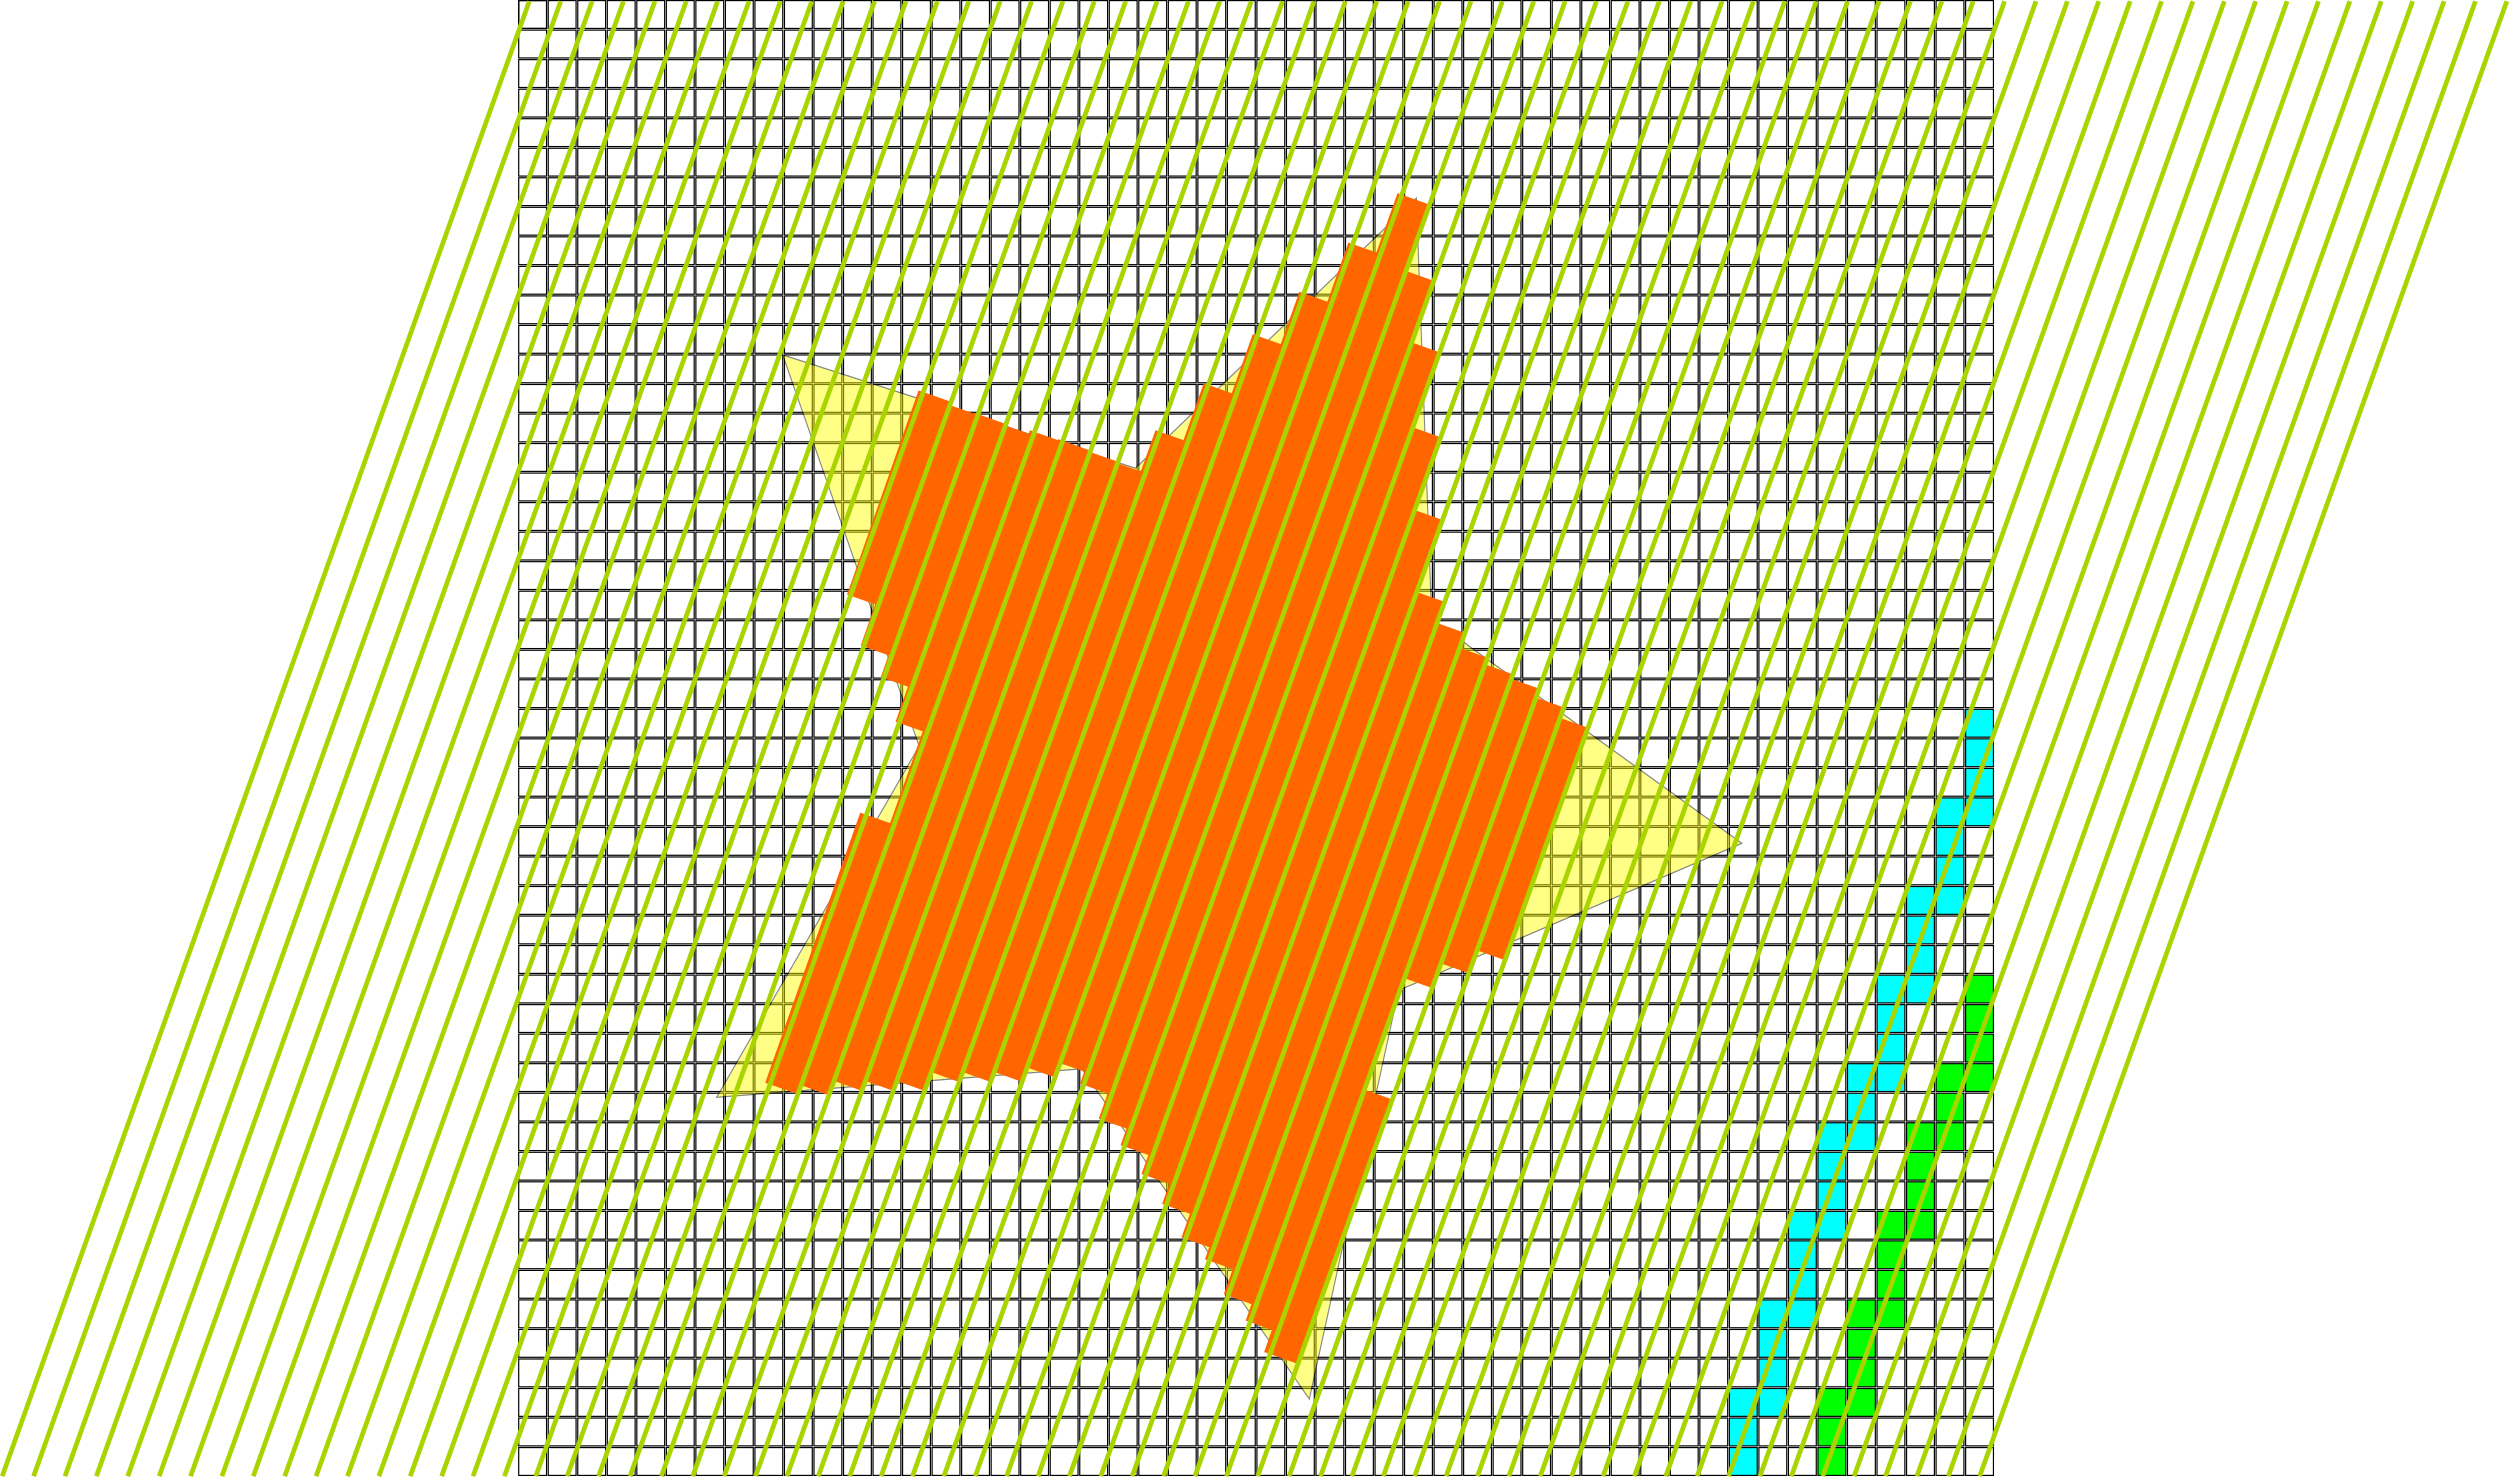
\includegraphics[width=0.5\textwidth]{../Vorgehensweise/drawings/ueberlappendeBahnen.png}
	\caption{Überlappende Landebahnen, die zu einem komplexen Polygon zusammengefasst werden können}
\end{figure}
Dieser Landebahnen-Merge ist wegen seiner intensiven Zugriffe auf die Datenbank auch in der Codebasis des Database Managers integriert. Es handelt sich aber um eine völlig unabhängige Komponente, welche auch in einem eigenen Prozess gestartet wird. Dieser unabhängige Postprocessing Task, durchsucht die Datenbank vollständig nach überlappenden Landebahnen mit gleicher Ausrichtung. Solche rechteckigen Bahnen können zu einer größeren Landefläche mit einem komplexen Polygon als Umriss zusammengefasst werden. 

Der Algorithmus ist sehr einfach gehalten: Nacheinander werden alle unbearbeiteten Bahnen aus der Datenbank gesucht. Für jede gefundenen Bahn wird eine weitere Datenbank-Abfrage gestartet um überlappende Bereiche gleicher Himmelsrichtung zu finden. Alle so erhaltenen überlappenden Bereiche werden über die Bibliothek \emph{turf.js} zu einem komplexen Polygon zusammengefasst. Als Parameter erhält dieses Feld die minimale Bahnlänge der beteiligten Ausgangsbahnen und die maximale Varianz und Steigung. Die ursprünglich von der Search Engine gelieferten Bahnen werden nicht aus der Datenbank entfernt, sondern lediglich als schon bearbeitet markiert. So kann jederzeit auf die originale Datenbasis zurückgegriffen werden.

Aktuell muss der Merge-Lauf noch manuell gestartet werden.

\section{Komponente "'landingClient"'}

Da in unserer Arbeitsgruppe bisher keine Erfahrung mit nativer GUI-Pro\-gram\-mierung vorliegt, wurde beschlossen, diesen Schritt auszulassen und direkt eine plattformunabhängige GUI basierend auf modernen Webtechnologien zu erstellen.

Diese GUI läuft auf jedem modernen Webbrowser und kann somit auch als Anzeige-Komponente auf schmalbrüstigen Geräten wie z. B. Smartphones zum Einsatz kommen, während das Heavy Lifting der Durchmusterung und der Datenhaltung auf einem kräftigen Server erledigt werden kann.

\begin{figure}[ht]
	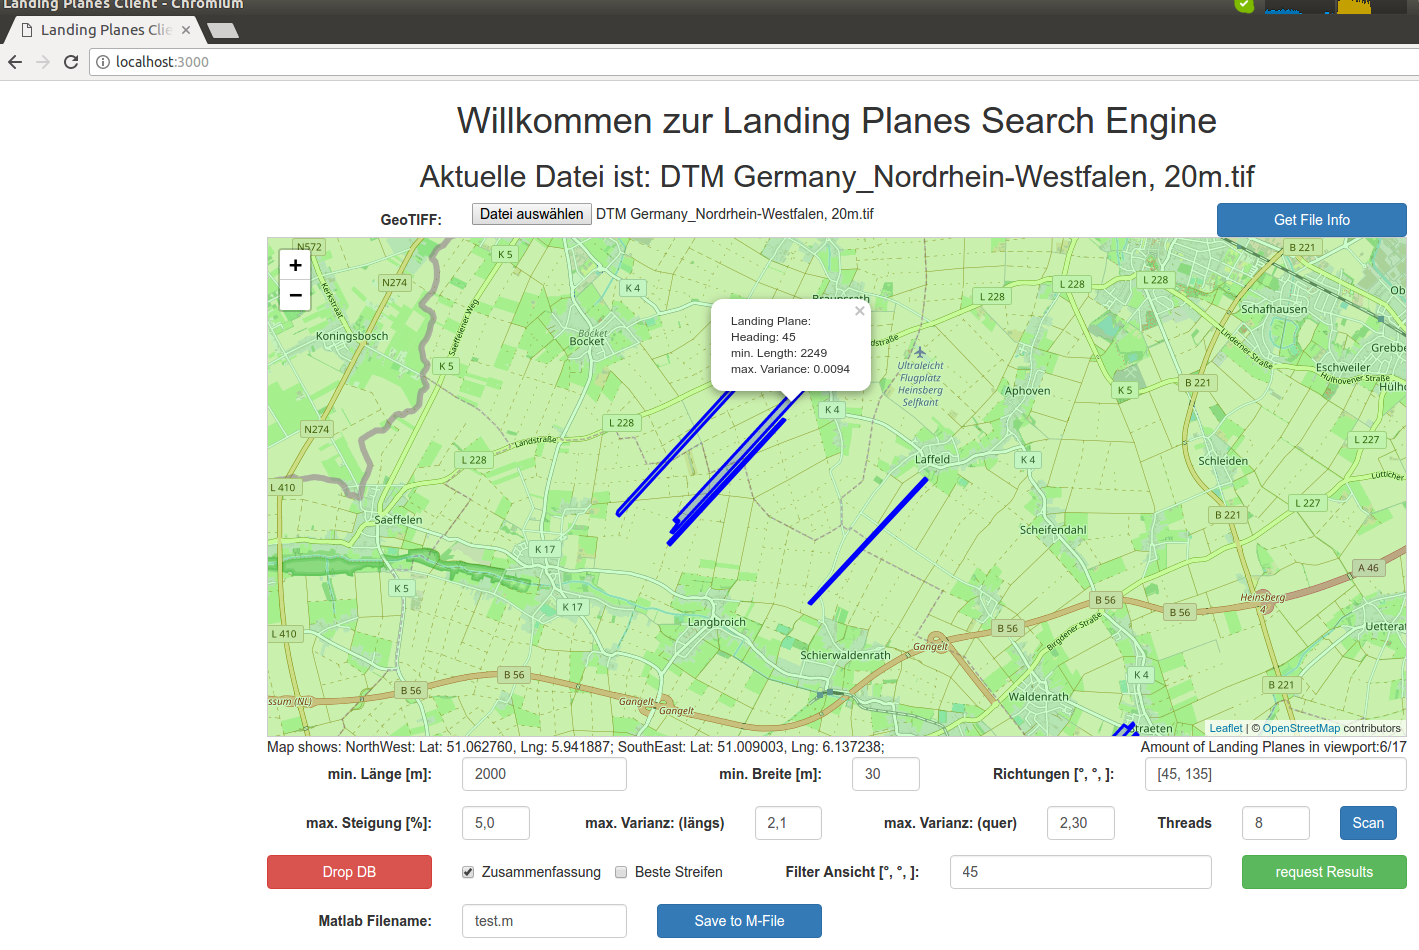
\includegraphics[width=\textwidth]{./drawings/LandingClient_Screen1.png}
	\caption{Beisiel Screenshot aus der Weboberfläche zur Bedienung des Systems}
\end{figure}

\subsection{Überblick}

Zur Realisierung der GUI wurde auf das von Facebook entwickelte und zur Verfügung gestellte REACT-Framework\footnote{siehe dazu: \href{https://facebook.github.io/react/}{https://facebook.github.io/react/}} zurückgegriffen. Der innere Status der Web-App wird über das dazu passende REDUX-State-Management\footnote{siehe dazu: \href{http://redux.js.org/}{http://redux.js.org/}} verwaltet. Die Darstellung der einzelnen HTML-Elemente erfolgt über die Bootstrap-Bibliothek\footnote{siehe dazu: \href{https://getbootstrap.com/}{https://getbootstrap.com/} und \href{https://react-bootstrap.github.io/}{https://react-bootstrap.github.io/}} von Twitter. Zur Darstellung der Karte wird auf die Bibliothek Leaflet\footnote{siehe dazu: \href{http://leafletjs.com/}{http://leafletjs.com/} und \href{https://github.com/PaulLeCam/react-leaflet}{https://github.com/PaulLeCam/react-leaflet}} zurückgegriffen, die eine einfache Darstellung von OpenStreetMap\footnote{siehe dazu: \href{https://www.openstreetmap.org}{https://www.openstreetmap.org}}-Karten erlaubt

REACT-Apps werden vollständig in Javascript kodiert, in das HTML-Ele\-mente eingebettet werden. 

Ohne auf zu viele Details einzugehen, wird die Funktionsweise der App lediglich kurz umrissen:

Die App unterhält intern einen State-Container (REDUX-Store), welcher alle notwendigen Daten enthält um den aktuellen Status und das darauf basierende Rendering der App zu bestimmen. In unserem Fall werden dort Informationen über die ausgewählte GeoTIFF-Datei (Dateiname, Dateieigenschaften, enthaltene Geodaten, Ausdehnung, \ldots) und die aktuell verfügbaren Notlandefelder (Array von \texttt{landingPlanes[]} mit GeoJSON als Inhalt) gehalten. 

\begin{figure}[ht]
	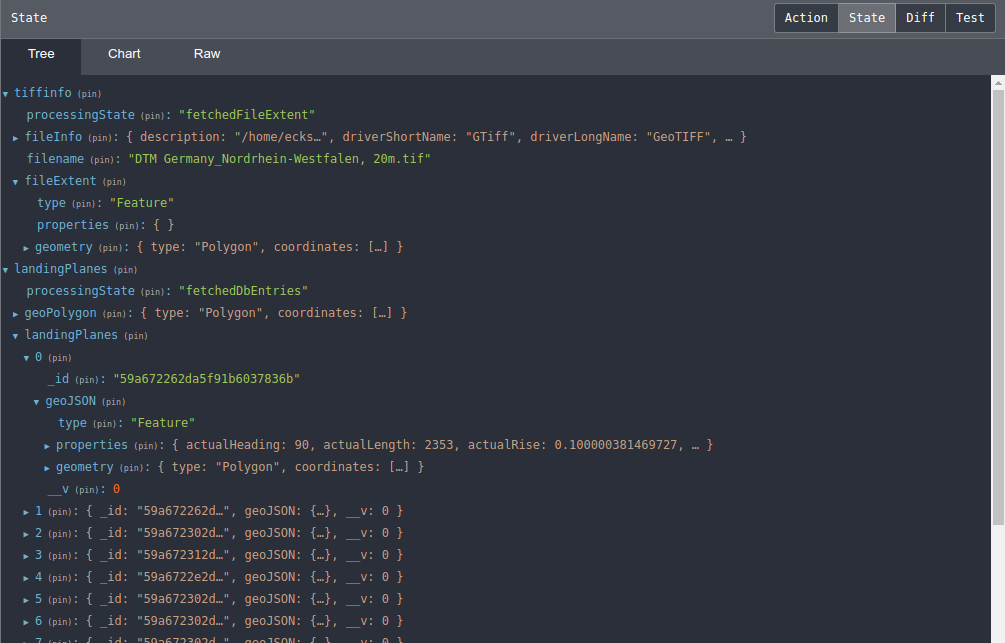
\includegraphics[width=\textwidth]{./drawings/ReduxStore_1.png}
	\caption{Der REDUX-Store zur Kontrolle des App-Status}
\end{figure}


Diese Daten werden nach Anforderung über die Bedienelemente asynchron vom Server (Database Manager per HTTP) abgefragt. Sobald eine asynchrone Anfrage beantwortet wurde sorgt das REACT-Framework dafür, dass die notwendigen Elemente des User-Interface neu gerendert werden um jederzeit eine aktuelle Darstellung zu erhalten. Diese Elemente werden mit dem REDUX-Store verknüpft, so dass auf Änderungen des Status direkt reagiert werden kann.

Zur Darstellung der gefundenen Landebahnen werden immer nur diejenigen Bahnen vom Server abgerufen, die im gezeigten Kartenausschnitt liegen. Das dient dazu, dass einerseits nicht zu viele (irrelevante) Daten über das Netzwerk übertragen werden müssen und sorgt gleichzeitig für eine relativ hohe Update Rate der Daten, da nach jedem Ändern von Ausschnitt oder Zoom eine Aktualisierung angefragt wird. Lokal im Client werden die angezeigten Daten noch gefiltert, so dass die Darstellung auf Bahnen bestimmter Richtungen eingeschränkt werden kann und der Benutzer auswählen kann, ob die zusammengefassten Landeflächen oder die einzelnen Rohdaten angezeigt werden sollen. Auch kann gefiltert werden ob die Teilbahnen minimaler Varianz überblendet werden sollen.



\subsection{Features und Bedienung}


Der Webclient für die Landebahnensuche präsentiert sich sehr schlicht. Zunächst wird lediglich eine leere Seite zur Auswahl der interessierenden GeoTIFF Datei dargestellt.

\begin{figure}[ht]
	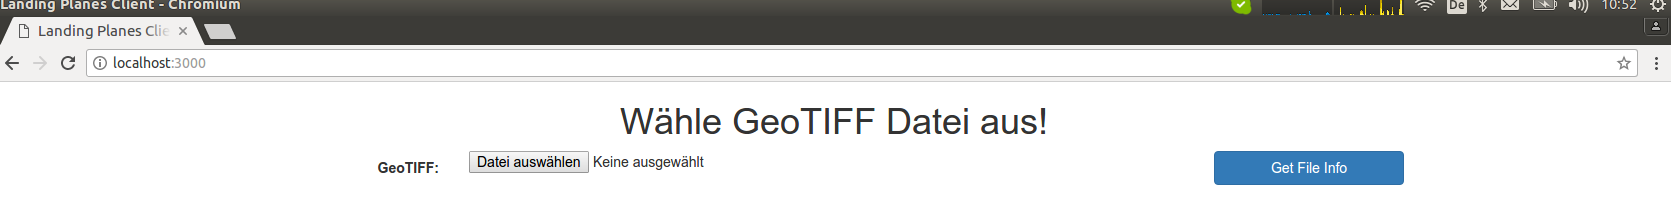
\includegraphics[width=\textwidth]{./drawings/LandingClient_Screen_Start.png}
	\caption{Auswahl der zu bearbeitenden GeoTIFF-Datei}
\end{figure}

Der Benutzer kann hier eine zu bearbeitende Datei auswählen und die zugehörigen Dateiinfos abrufen.

Die Darstellung wechselt zur Hauptansicht, in welcher der in der ausgewählten Datei enthaltene Ausschnitt in einer Karte angezeigt wird.
\begin{figure}[ht]
	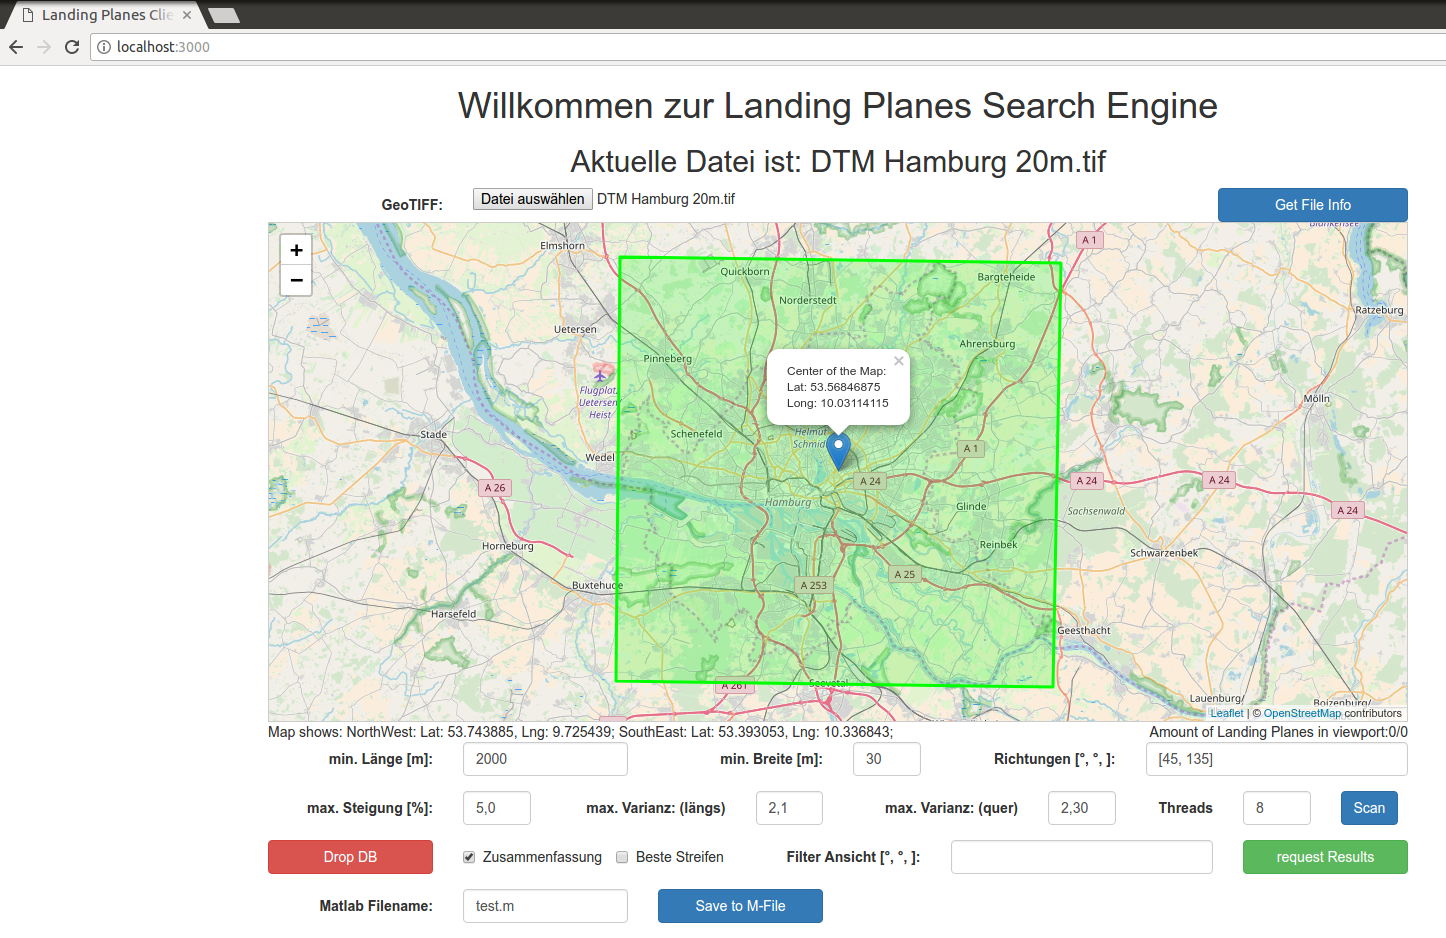
\includegraphics[width=\textwidth]{./drawings/LandingClient_Screen_Ueberblick.png}
	\caption{Überblick über den im GeoTIFF enthaltenen Datensatz}
\end{figure}

Hier kann der Benutzer die relevanten Parameter zu minimalen Bahnmaßen und Steigungs- und Holprigkeitseigenschaften einstellen. Auch die Durchmusterungsrichtungen können hier vorgegeben werden. Ein Klick auf "`Scan"' setzt einen "`SCAN"'-Task über die REST-API des Servers ab. Als Scan-Bereich wird der gerade sichtbare Bereich der Karte angegeben. Wenn die Kartenausschnitt größer ist als der GeoTIFF-Datensatz, dann wird natürlich nur der vorhandene Datensatz untersucht.

Leider wird die Fertigstellung des Scan-Tasks noch nicht per Push an den Client zurückgemeldet. Daher ist ein "`request Results"' Knopf vorhanden, der eine manuelle Abfrage der gefundenen Bahnen erlaubt. Diese Anfrage wird aber auch bei jeder Manipulation des gezeigten Kartenausschnitts abgesetzt, so dass eine manuelle Abfrage nur selten notwendig ist.

Sobald potentielle Bahnen angezeigt werden, kann der Benutzer darauf noch Filter anwenden, um die Darstellung übersichtlicher zu gestalten.

\begin{figure}[ht]
	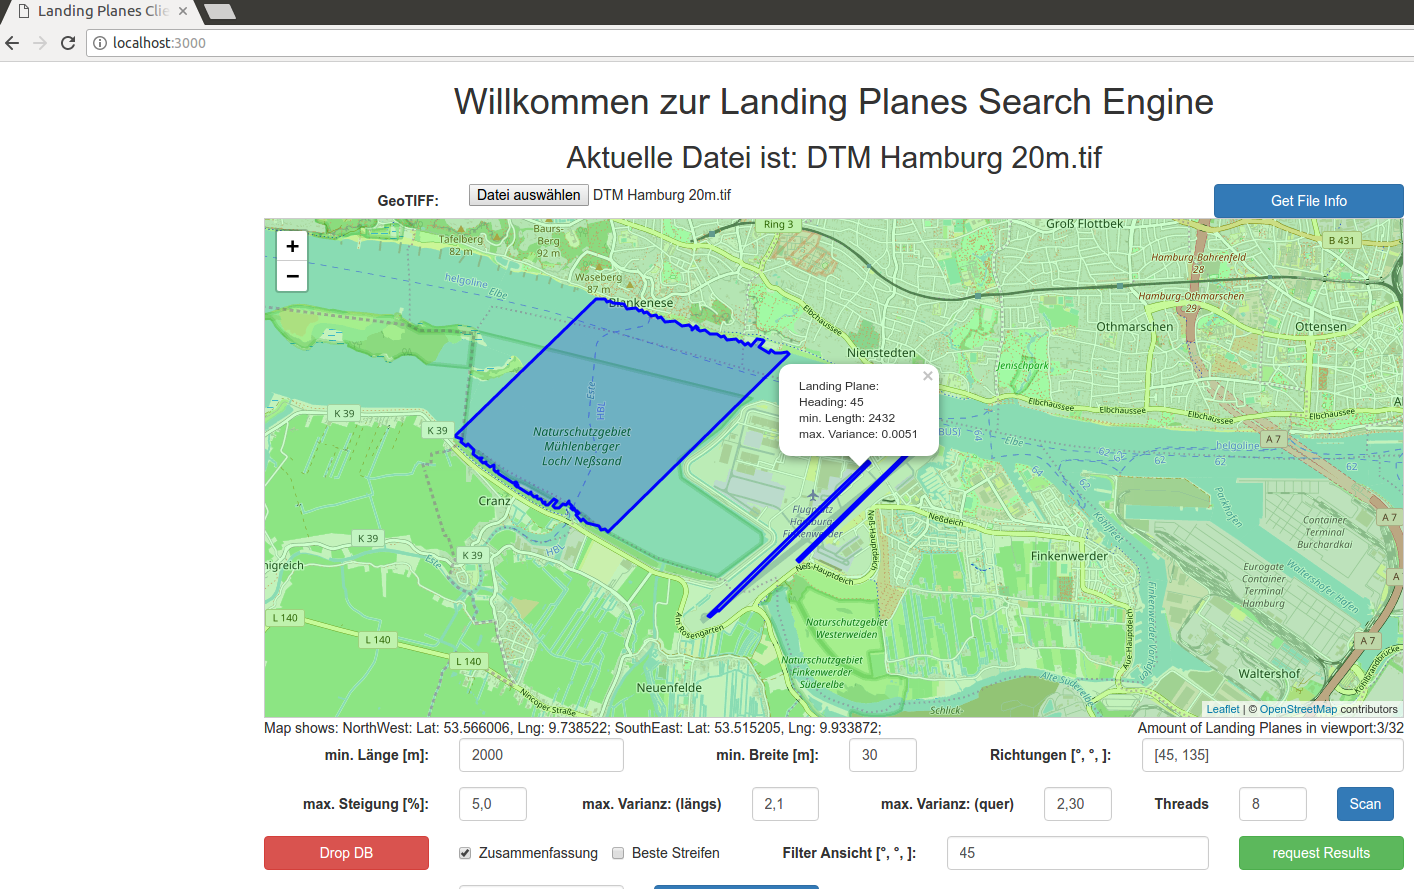
\includegraphics[width=\textwidth]{./drawings/LandingClient_Screen_Planes.png}
	\label{dargestellte_bahnen}
	\caption{Gefundene Landebahnen mit angewendeten Filtern zur Darstellung}
\end{figure}

\section{Ausblick und weitere Ideen}

Im Rahmen der Untersuchungen mit der im Praktikum erarbeiteten Softwarelösung sind einige verblüffende und interessante Artefakte sichtbar geworden.
Unabhängig von dem Winkel der Landebahn zeigte sich, dass der südöstliche Teil von NRW keine geeigneten Landebahnen bietet. Dies ist der Tatsache geschuldet, dass dort Gebirgszüge wie das Süderbergland und das Sauerland zu finden sind.
Entlang der niederländischen Grenze und an der Grenze zu Niedersachsen ist das Gebiet flacher.
Weiterhin ist überraschend, dass die ca. 100 Mio Datenpunkte in so kurzer Zeit und mit so wenig Speicherbedarf bearbeitet werden können. Selbst auf einer kleinen virtuellen Maschine lief die Durchmusterung sehr zügig.
Weiterhin war überraschend, dass die Programmübersetzung mit optimiertem Code eine extreme Beschleunigung brachte.
Diese konnte durch das Threading noch weiter gesteigert werden.
Allerdings zeigt sich auch, dass vermutlich schon bei recht kleiner Parallelität (4-fach parallel) der Speed-up nicht mehr linear mit der Anzahl der Prozessoren korreliert.
Die Berechnung der Varianz der Landebahn bzw. das Auffinden der optimalen Landebahnen aus einer Fläche benötigt in sich schon relativ viele Rechenoperationen. Hier könnte nochmals eine feingranulare Parallelisierung vorgenommen werden.
Es könnten weitere Parameter eingeführt werden, um noch mehr Randbedingungen an die Qualität einer Landebahn zu stellen. Dieses benötigt aber sicherlich noch mehr domänenpezifischen Input.
Interessant wäre es, Datensets mit mehr Datenpunkten und die Laufzeit bei diesen Randbedingungen zu untersuchen. Insbesondere, wenn die Fläche in eine größere Anzahl von Subkacheln gesplittet wird.

\skippingparagraph

Zu Ende diese Berichts sollen noch einige konkrete Ideen angegeben werden, welche weitere Verbesserungen des vorgestellten Systems realisieren würden. Bei einer weiteren Bearbeitung des Themas müsste bewertet werden, welche dieser Ideen den größten Nutzen bringen.
 
\subsection{Parallele Bearbeitung mehrerer Kacheln per MPI}
Besonders bei größeren Datensätzen wäre es interessant, die Laufzeiteigenschaften der Software zu untersuchen. Bei sehr großen Datensätze wäre ein embedding in eine MPI Lösung vielleicht interessant, das die Daten innerhalb eines Clusters verteilt. Pro Knoten könnte dann mit Threading eine feingranulare Parallelisierung durchgeführt werden. 

Die im GeoTIFFHandler sowieso schon vorgesehen Kachelung des Datensatzes könnte direkt zur Aufteilung der Daten auf verschiedene MPI-Knoten genutzt werden. Die Durchmusterung dieser einzelnen Kacheln kann völlig unabhängig voneinander erfolgen, so dass mit einem linearen Speedup gerechnet werden kann, solange die Datensätze große genug sind.

\subsection{Richtungskorrektur des GeoTIFF}

Wie weiter oben schon erwähnt, stimmt aktuell die Ausrichtung der Landebahnen nicht mit der tatsächlichen Ausrichtung auf der Erdkugel überein. Es entsteht eine geringe Abweichung, da für diesen Proof-of-concept angenommen wurde, dass der GeoTIFF-Datensatz strikt in Nord-Süd- und Ost-West-Richtung ausgerichtet ist. Genau genommen muss aber die korrekte Ausrichtung eines jeden Pixels einzeln bestimmt werden um die korrekte auf Kugelkoordinaten bezogene Ausrichtung zu erhalten.

In der \emph{GDAL}-Bibliothek stehen alle benötigten Transformationen zur Verfü\-gung um die korrekte Ausrichtung für jedes Pixel zu berechnen. Die Berechnung innerhalb der Duchmusterungsroutine würde damit jedoch erheblich aufwändiger, weil in jedem Schritt der nächste Nachbar neu berechnet werden muss und nicht mehr ein vorberechneter Richtungsvektor zum Fortschreiten entlang eines Durchmusterungsstrahls in Pixelkoordinaten verwendet werden kann. Es wäre interessant zu untersuchen, ob eine Richtungskorrektur wirklich bei jedem Rasterpixel notwendig wird, oder ob eine seltenere Richtungskorrektur nicht ausreichend gute Ergebnisse liefert.

\subsection{Push für Webclient}
Aktuell müssen die Ergebnisse einer Durchmusterung noch manuell vom Server in den Web-Client abgerufen werden. Um den Komfort zu steigern wäre es schön einen Push-Mechanismus zu implementieren, der den Client benachrichtigt, sobald neue Objekte in der Datenbank eingetragen werden.

Ein solcher Mechanismus ist über Web-Sockets\footnote{siehe hierzu: Als Einstieg \href{https://de.wikipedia.org/wiki/WebSocket}{https://de.wikipedia.org/wiki/WebSocket} und zur konkreten Implementierung in einer Express-App  \href{https://www.npmjs.com/package/express-ws}{https://www.npmjs.com/package/express-ws}.} leicht verfügbar. Damit kann der Server an registrierte Clients Push-Nachrichten senden, ohne dass eine neue Abfrage abgesetzt werden muss.


\subsection{Merge als nachgeschalteter Prozess aus dem Speicher}
Der Merge der überlappenden Landebahnen ist aktuell sehr simpel und wenig effizient implementiert. Bei einer großen Menge frisch gefundener Landebahnen dauert der Merge-Lauf aktuell deutlich länger als die Durchmusterung des zugrunde liegenden GeoTIFF. Das liegt daran, dass in der aktuellen Implementierung eine sehr große Anzahl an Datenbankzugriffen stattfindet: Es wird jede unbearbeitete Landebahn aus der Datenbank einzeln abgefragt. Daraufhin werden zu jeder so gefundenen Bahn alle überlappenden Objekte in der Datenbank gesucht. Das neu entstehende Polygon wird nun als neues, unbearbeitetes Objekt in der Datenbank gespeichert. Für jedes so bearbeitete Objekt müssen sowohl Lese- als auch Schreibzugriffe auf der Datenbank stattfinden.

Sehr viel effizienter ließe sich ein Merge-Postprocessing implementieren, wenn die neu gefundenen Bahnen eines Scan-Durchlaufs im Speicher gehalten würden, und nach Beendigung des Scan-Durchlaufs ein Merge über die Objekte im Speicher durchgeführt würde. Die damit gewonnenen zusammengefassten Landeflächen können mit einem einzigen Datenbankzugriff geschrieben werden. 

Mit einem solchen Postprocessing ohne Datenbankzugriffe sind Performance Steigerung beim Merge um Größenordnungen zu erwarten.
Ob der Merge in C++ oder in JavaScript implementiert wird, dürfte nach erster Einschätzung keine große Rolle spielen.

\subsection{Kollisionsabfrage mit Objekten aus OSM}
Wie in Abbildung \ref{dargestellte_bahnen} zu erkennen ist findet eine Durchmusterung natürlich bevorzugt Wasserflächen als potentielle Landeflächen, da diese in den Höhendaten sehr flach und glatt erscheinen. Obwohl es Piloten gibt, die auch auf Wasser landen können\footnote{siehe hierzu: \href{http://www.zeit.de/wissen/2016-09/chesley-sullenberger-new-york-airbus-pilot-hudson-river-notlandung}{http://www.zeit.de/wissen/2016-09/chesley-sullenberger-new-york-airbus-pilot-hudson-river-notlandung}}, so ist das in der Regel nicht die bevorzugte Landebahn. 

Als Erweiterung der Landebahnensuche kann relativ einfach eine Kollisionsabfrage mit unerwünschten Objekten eingebaut werden. Diese unerwünschten Objekte müssen lediglich in einer Datenbank als GeoJSON vorliegen. Vor dem Eintrag einer neuen Bahn kann geprüft werden, ob eine Kollision mit einem dieser Sperr-Objekte vorliegt. Falls das der Fall ist so kann die neue Bahn gegebenenfalls vollständig verworfen, oder aber beschnitten werden.

Geeignete Sperrflächen sind prinzipiell über die Datenbank von Openstreetmap verfügbar. 

Um diese Funktionalität zu implementieren, sind jedoch noch deutlich weitergehende Untersuchungen über Art und Datenformat unerwünschter Objekte durchzuführen.

\appendix
\section{Installationsanleitung}

Um die hier beschriebene Software auszuprobieren ist ein Rechner mit einer aktuellen Linux-Distribution erforderlich.
Notwendig ist insbesondere:
\begin{itemize}
\item eine aktuelle Installation von Node.js ($\geq$ Version 8)
\item eine aktuelle Installation von NPM
\item eine aktuelle installation von bower (\texttt{npm install -g bower})
\item eine aktuelle Version der gdal-Library, deren Header-Dateien unter \texttt{/usr/include/gdal} liegen müssen
\item eine aktuelle Version des kompilierten \texttt{gdal-bin} Pakets (insbesondere \texttt{gdalinfo} im PATH)
\item eine laufende Instanz einer MongoDB, welche sich auf \texttt{mongodb://localhost:27017} ansprechen lässt
\end{itemize}

Zunächst wird das gesamte Projekt von Github auf den Rechner geklont:
\begin{verbatim*}
git clone git@github.com:opt12/LandingPlanes.git
\end{verbatim*}

\skippingparagraph
Dann muss die Search Engine Komponente %in zwei Schritten 
gebaut werden:

%Zunächst die Bibliothek zur Durchmusterung
%\begin{verbatim*}
%cd LandingPlanes/src/Durchmusterung
%make all
%\end{verbatim*}
%
%Hierbei wird auch die passende GDAL-Bibliothek aus dem Netz heruntergeladen und in den Ordner \texttt{./gdal} gespeichert und gebaut. \footnote{Es kann vorkommen, dass beim Build der Bibliothek ein Fehler auftritt (wenn eine ältere Version von Anaconda auf dem Rechner installiert ist.). In diesem Fall ist es meist ausreichend die GDAL Bibliothek in dem Zustand zu benutzen, den sie bis zum Fehler hat und die \texttt{plane\_library.a} nochmals manuell zu bauen:\\
%\texttt{cd LandingPlanes/src/Durchmusterung}\\
%\texttt{make ./lib/plane\_library.a}
%}

Die \texttt{1597\_searchEngine} Komponente und die Bibliotheken \texttt{plane\_library.a} und \texttt{libGeoTiffHandler.a} können gemeinsam erstellt werden:\footnote{In den Verzeichnissen \texttt{LandingPlanes/src/Durchmusterung} und \texttt{LandingPlanes/src/GeoTiff\_Handler} befinden sich auch Makefiles um die statischen Bibliotheken einzeln zu bauen.}
\begin{verbatim*}
cd LandingPlanes/src/1597_searchEngineWrapper/
make
\end{verbatim*}

\skippingparagraph
Nun muss der Landing Client gebaut werden.
\begin{verbatim*}
cd LandingPlanes/src/1597_LandingClient
npm install
bower install
npm run local-build
\end{verbatim*}

Es ist nun eine Datei \texttt{LandingPlanes/src/1597\_LandingClient/bundle.js} erstellt worden.

\skippingparagraph
Als letzte Komponente muss der Database Manager vorbereitet werden.
\begin{verbatim*}
cd LandingPlanes/src/1597_DatabaseManager
npm install
\end{verbatim*}

\skippingparagraph
Nun muss lediglich die Datei \texttt{LandingPlanes/src/1597\_DatabaseManager/package.json} überprüft und gegebenenfalls angepasst werden. Es müssen die Pfade im Skript 
\begin{verbatim*}
"start": "node ./bin/www --tiffpath=/home/eckstein/dev/LandingPlanes/terrain
         --wrapper=../1597_searchEngineWrapper/bin/1597_searchEngineWrapper 
         --clientpath='../1597_LandingClient'"
\end{verbatim*}
angepasst werden.

\texttt{tiffpath}: Ist der Pfad zu den GeoTIFF Dateien. (Der muss gesetzt werden, da aktuell nur der Dateiname übergeben wird, nicht der Pfad)

\texttt{wrapper}: Ist der Pfad zur kompilierten Wrapper-Applikation. Diese wird automatisch gestartet und über einen Unix-Socket mit Daten gefüttert. 

\texttt{clientpath}: Der Pfad zum Verzeichnis für die React-Applikation, also den 1597\_LandingClient.

\texttt{terminal}: Ist ein optionaler Parameter um festzulegen, welche Terminal-Emulation benutzt werden soll. \texttt{xterm} sollte auf allem Maschinen funktionieren, falls der Defaultwert \texttt{gnome-terminal} nicht verfügbar ist. Der Parameter kann dann noch mit \texttt{--terminal='xterm'} hinzugefügt werden.

\skippingparagraph
Wenn diese Vorbereitungen abgeschlossen sind, kann das System mit
\begin{verbatim*}
cd LandingPlanes/src/1597_DatabaseManager
npm start
\end{verbatim*}

gestartet werden und über das Öffnen von \href{http://localhost:3000}{http://localhost:3000} bedient werden.


\skippingparagraph
Ein manueller Merge von überlappenden Landebahnen kann angestoßen werden, wenn in einem eigenen Terminal das npm-Skript \texttt{cleanup} aufgerufen wird:
\begin{verbatim*}
cd LandingPlanes/src/1597_DatabaseManager
npm run cleanup
\end{verbatim*}



\end{document}
